\documentclass[10pt,oneside,titlepage,final]{book}
% lingua
\usepackage[utf8]{inputenc}
\usepackage[T1]{fontenc}
\usepackage{lmodern}
\usepackage[italian]{babel}
\usepackage[babel]{csquotes}

\usepackage[mark]{gitinfo2}

% ambienti math
\usepackage{amsmath}
\usepackage{amsthm}
\usepackage{amsfonts}
\usepackage{amssymb}
\usepackage{thmtools}
\usepackage{cancel}
\usepackage{bm}
\usepackage{siunitx}

% indici acronimi bibliografia
%\usepackage{makeidx}
%\usepackage[backend=biber]{biblatex}
\usepackage{multicol}
\usepackage{acronym}

% diagrammi circuiti elettrici
\usepackage[siunitx]{circuitikz}

% grafica
\usepackage{graphicx}
\usepackage{xcolor}
\usepackage{pgfplots,pgfplotstable}
\pgfplotsset{compat=1.12,/tikz/prefix=plots/}
\usetikzlibrary{math,matrix,chains}
\usetikzlibrary{scopes,positioning,fit,intersections}
\usetikzlibrary{angles,shapes,arrows,patterns,fadings}
\usetikzlibrary{decorations.pathreplacing,decorations.pathmorphing,decorations.markings,decorations.shapes}
\usetikzlibrary{tikzmark}
\usepgfplotslibrary{fillbetween,patchplots}
\pgfplotsset{every linear axis/.append style={axis lines=middle,enlargelimits}}
\pgfplotsset{trig format plots=rad}
\pgfplotsset{/pgfplots/colormap={graywhite}{gray=(0.75) gray=(1.0)}}

% oriented lines
% Thanks: http://tex.stackexchange.com/questions/163689/add-arrows-to-a-smooth-tikz-function
\tikzset{
    set arrow inside/.code={\pgfqkeys{/tikz/arrow inside}{#1}},
    set arrow inside={end/.initial=>, opt/.initial=},
    /pgf/decoration/Mark/.style={
        mark/.expanded=at position #1 with
        {
            \noexpand\arrow[\pgfkeysvalueof{/tikz/arrow inside/opt}]{\pgfkeysvalueof{/tikz/arrow inside/end}}
        }
    },
    arrow inside/.style 2 args={
        set arrow inside={#1},
        postaction={
            decorate,decoration={
                markings,Mark/.list={#2}
            }
        }
    },
}

% icone creative commons
\usepackage{ccicons}

% float and figure
\usepackage{float}
\usepackage{subfig}
\usepackage{caption}
\captionsetup{tableposition=top,figureposition=bottom,font=small,format=hang}
\usepackage{booktabs}
\usepackage{tablefootnote}
\renewcommand{\thefootnote}{\fnsymbol{footnote}}
\newcommand{\footnoteref}[1]{\textsuperscript{\ref{#1}}}

% hyperlink
\usepackage{hyperref}
\hypersetup{
	pdfauthor={Giovanni Grieco},
	pdftitle={Appunti di Fondamenti di Automatica},
	pdfsubject={Modulo I - Analisi dei Sistemi di Controllo},
	pdfencoding=auto,
	psdextra,
	colorlinks,
	linkcolor={black},
	citecolor={blue!50!black},
	urlcolor={blue!80!black}
}

% definizioni nuovi stili teoremi
\theoremstyle{definition}
\newtheorem{definizione}{Definizione}[chapter]
\newtheorem{esempio}{Esempio}[chapter]
\newtheorem{esercizio}{Esercizio}[chapter]
\newtheorem{nota}{Nota}[chapter]
\newcommand{\keyword}[2][]{\textsc{#2}\index{#1}}

% fix: Warning Font shape for text `textbullet' undefined (Font)
\renewcommand\textbullet{\ensuremath{\bullet}}

% Simboli matematici di default
\renewcommand\epsilon{\varepsilon}


% formato pagina - iPad 9.7"
\usepackage[
	paperwidth=14.8cm,
	paperheight=19.8cm,
	width=14.75cm,
	height=19.40cm,
	left=0.03cm
]{geometry}

% frontespizio Poliba
\usepackage{polibatitle}
\title{Appunti di \\ Fondamenti di Automatica}
\professor[f]{M.P. Fanti}
\assistant{Ing. G. Pedroncelli}

\makeindex

\begin{document}
\hypersetup{pageanchor=false}
\frontmatter
\maketitle
\newpage

\null\vspace{\stretch{3}}\null
\vfill\noindent
\textbf{Contributori:} \input{contributori} \\
\textbf{Join us!} \url{https://github.com/corsaroquad/poliba-automatica}
\hspace*{\fill}\ccbyncsa

\cleardoublepage\clearpage{\pagestyle{empty}\cleardoublepage}

\pagenumbering{gobble}

% indice contenuti
\tableofcontents

\mainmatter
\pagenumbering{gobble}
\renewcommand\partname{Modulo}

\part{Analisi dei Sistemi di Controllo}
% TODO: Prima parte - prima dell'esonero di novembre
\chapter{Diagrammi a blocchi}

I diagrammi a blocchi servono per descrivere in modo astratto i sistemi automatici.
È possibile descrivere all'interno del blocco una propria \emph{funzione di trasferimento},
e questa sarà preceduta da delle \emph{frecce entranti} che faranno da \emph{input} e
da delle \emph{frecce uscenti} che faranno da \emph{output}.

Ogni input e output, secondo la logica del sistema, può essere sommato o sottrato con
altri fattori, come altri input e/o output oppure disturbi.
Il seguente esempio mostra un sistema statico con solo un input e un output.
\begin{center}\begin{tikzpicture}[auto, node distance=2cm,>=latex']
	\node [input, name=rinput] (rinput) {};
	\node [block, right of=rinput] (controller) {\(G(s)\)};
	\node [output, right of=controller, node distance=2cm] (output) {};
	\draw [->] (rinput) -- node{\(X(s)\)} (controller);
	\draw [->] (controller) -- node [name=y] {\(Y(s)\)}(output);
\end{tikzpicture}\end{center}

In caso di strutture più complesse e con l'interazione di più grandezze si parla
di \emph{sistema interconnesso}.

Esistono diverse relazioni che regolano la struttura dei diagrammi a blocchi,
di seguito elencate e con i rispettivi metodi per poterli semplificare.

\section{Strutture equivalenti}
\subsection{Blocchi in parallelo}
\begin{center}\begin{tikzpicture}[auto, node distance=2cm,>=latex']
	\node [input, name=xinput] (xinput) {};
	\node [block, right of=xinput] (ctrl1) {\(G_1(s)\)};
	\node [block, below of=ctrl1, node distance=2cm] (ctrl2) {\(G_2(s)\)};
	\node [sum, right of=ctrl1, node distance=2cm] (sum) {};
	\node [output, right of=sum] (output) {};
	\draw [->] (xinput) -- node[name=z]{} node{\(X(s)\)} (ctrl1);
	\draw [->] (ctrl1) -- node[name=out1] {\(Y_1(s)\)} (sum);
	\draw [->] (z) |- (ctrl2);
	\draw [->] (ctrl2) -| node[pos=0.25,anchor=south]{\(Y_2(s)\)} (sum);
	\draw [->] (sum) -- node[] {\(Y(s)\)} (output);
\end{tikzpicture}\end{center}

Le equazioni espresse nello schema sono
\begin{align*}
	Y_1(s) &= G_1(s)\,X(s) \\
	Y_2(s) &= G_2(s)\,X(s) \\
	Y(s) &= Y_1(s) + Y_2(s) \\
	\implies Y(s) &= \sum_{i=1}^\infty G_i(s)\,X(s)
\end{align*}
e quindi si può semplificare lo schema con un unico blocco che ne faccia la somma:
\begin{center}\begin{tikzpicture}[auto, node distance=2cm,>=latex']
	\node [input, name=x] (x) {};
	\node [block, right of=x] (ctrl) {\(\sum_{i=0}^\infty G_i(s)\)};
	\node [output, right of=ctrl] (y) {};
	\draw [->] (x) -- node[]{\(X(s)\)} (ctrl);
	\draw [->] (ctrl) -- node[]{\(Y(s)\)} (y);
\end{tikzpicture}\end{center}

Si conclude che \emph{il parallelo di due o più blocchi è equivalente alla somma
algebrica delle f.d.t. (guadagni) dei rispettivi blocchi interessati}.

\subsection{Blocchi in cascata o in serie}
\begin{center}\begin{tikzpicture}[auto, node distance=2cm,>=latex']
	\node [input, name=x] (x) {};
	\node [block, right of=x] (ctrl1) {\(G_1(s)\)};
	\node [block, right of=ctrl1, node distance=3cm] (ctrl2) {\(G_2(s)\)};
	\node [output, right of=ctrl2] (y) {};
	\draw [->] (x) -- node[]{\(X(s)\)} (ctrl1);
	\draw [->] (ctrl1) -- node[]{\(Z(s)\)} (ctrl2);
	\draw [->] (ctrl2) -- node[]{\(Y(s)\)} (y);
\end{tikzpicture}\end{center}

Le equazioni espresse nello schema sono
\begin{align*}
	Y(s) &= G_2(s)Z(s) \\
	Z(s) &= G_1(s)X(s) \\
	\implies Y(s) &= \prod_{i=1}^\infty G_i(s)X(s)
\end{align*}
e quindi si può semplificare lo schema con un blocco che ne faccia il prodotto:
\begin{center}\begin{tikzpicture}[auto, node distance=2cm,>=latex']
	\node [input] (x) {};
	\node [block, right of=x] (ctrl) {\(\prod_{i=0}^\infty G_i(s)\)};
	\node [output, right of=ctrl] (y) {};
	\draw [->] (x) -- node[]{\(X(s)\)} (ctrl);
	\draw [->] (ctrl) -- node[]{\(Y(s)\)} (y);
\end{tikzpicture}\end{center}

Si conclude che \emph{una serie di blocchi equivale al prodotto algebrico delle
f.d.t. dei rispettivi blocchi interessati}.

\subsection{Scambio di nodi sommatori}
\begin{center}\begin{tikzpicture}[auto, node distance=2cm,>=latex']
	\node [input] (x) {};
	\node [sum, right of=x] (sum1) {};
	\node [input, above of=sum1] (y) {};
	\node [sum, right of=sum1] (sum2) {};
	\node [input, above of=sum2] (w) {};
	\node [input, right of=sum2] (z) {};
	\draw [->] (x) -- node[]{\(X(s)\)} (sum1);
	\draw [->] (y) -- node[]{\(Y(s)\)} (sum1);
	\draw [->] (sum1) -- (sum2);
	\draw [->] (w) -- node[]{\(W(s)\)} (sum2);
	\draw [->] (sum2) -- node[]{\(Z(s)\)} (z);
\end{tikzpicture}\end{center}

L'equazione è \(Z(s) = W(s) + \bigl(Y(s) + X(s)\bigr)\) che, per la proprietà associativa
dell'addizione, può essere rivalutata come
\begin{align*}
	Z(s) &= \bigl(X(s) + W(s)\bigr) + Y(s) \\
	Z(s) &= \bigl(Y(s) + W(s)\bigr) + X(s) \\
	Z(s) &= X(s) + Y(s) + W(s)
\end{align*}
\begin{center}\begin{tikzpicture}[auto,node distance=2cm,>=latex']
	\begin{scope}
		\node [input] (x) {};
		\node [sum, right of=x] (sum1) {};
		\node [input, above of=sum1] (w) {};
		\node [sum, right of=sum1] (sum2) {};
		\node [input, below of=sum2] (y) {};
		\node [output, right of=sum2] (z) {};
		\draw [->] (x) -- node[]{\(X(s)\)} (sum1);
		\draw [->] (w) -- node[]{\(W(s)\)} (sum1);
		\draw [->] (sum1) -- (sum2);
		\draw [->] (y) -- node[]{\(Y(s)\)} (sum2);
		\draw [->] (sum2) -- node[]{\(Z(s)\)} (z);
	\end{scope}
	\begin{scope}[xshift=5cm]
		\node [input] (y) {};
		\node [sum, right of=y, node distance=2cm] (sum1) {};
		\node [input, below of=sum1] (w) {};
		\node [sum, right of=sum1] (sum2) {};
		\node [input, above of=sum2] (x) {};
		\node [output, right of=sum2] (z) {};
		\draw [->] (y) -- node[]{\(Y(s)\)} (sum1);
		\draw [->] (w) -- node[]{\(W(s)\)} (sum1);
		\draw [->] (sum1) -- (sum2);
		\draw [->] (x) -- node[]{\(X(s)\)} (sum2);
		\draw [->] (sum2) -- node[]{\(Z(s)\)} (z);
	\end{scope}
	\begin{scope}[xshift=11cm]
		\node [input] (x) {};
		\node [sum, right of=x, node distance=2cm] (sum) {};
		\node [input, above of=sum] (y) {};
		\node [input, below of=sum] (w) {};
		\node [output, right of=sum] (z) {};
		\draw [->] (x) -- node[]{\(X(s)\)} (sum);
		\draw [->] (y) -- node[]{\(Y(s)\)} (sum);
		\draw [->] (w) -- node[]{\(W(s)\)} (sum);
		\draw [->] (sum) -- node[]{\(Z(s)\)} (z);
	\end{scope}
\end{tikzpicture}\end{center}

Si conclude che \emph{l'ordine dei blocchi collegati ad un sommatore è ininfluente
e possono essere collegati da un unico blocco sommatore}.

\subsection{Spostamento di un punto di prelievo a monte di un blocco}
\begin{center}\begin{tikzpicture}[auto,node distance=2cm,>=latex']
	\node [input] (x) {};
	\node [block, right of=x] (ctrl) {\(G(s)\)};
	\node [output, right of=ctrl] (y) {};
	\node [output, below of=x, node distance=1cm] (yy) {};
	\draw [->] (x) -- node[]{\(X(s)\)} (ctrl);
	\draw [->] (ctrl) -- node[name=out]{\(Y(s)\)} (y);
	\draw [->] (out) |- node[pos=0.8]{\(Y(s)\)} (yy);
\end{tikzpicture}\end{center}

Questo schema, dato che ha per entrambe le uscite equazione \(Y(s) = G(s)X(s)\)
può essere sostituito dall'equivalente
\begin{center}\begin{tikzpicture}[auto,node distance=2cm,>=latex']
	\node [input] (x) {};
	\node [block, right of=x, node distance=4cm] (ctrl1) {\(G(s)\)};
	\node [output, right of=ctrl1] (y) {\(Y(s)\)};
	\draw [->] (x) -- node[name=align,pos=0.5]{\(X(s)\)} (ctrl1);
	\draw [] (x) -- node[name=in,pos=0.85]{} (ctrl1);
	\draw [->] (ctrl1) -- node[]{\(Y(s)\)} (y);
	% secondo livello
	\node [block, below of=align] (ctrl2) {\(G(s)\)};
	\node [output, left of=ctrl2, node distance=1.8cm] (yy) {};
	\draw [->] (in) |- (ctrl2);
	\draw [->] (ctrl2) -- node[]{\(Y(s)\)} (yy);
\end{tikzpicture}\end{center}

\subsection{Spostamento di un punto di prelievo a valle di un blocco}
\begin{center}\begin{tikzpicture}[auto,node distance=2cm,>=latex']
	\node [input] (x) {};
	\node [block, right of=x, node distance=3cm] (ctrl) {\(G(s)\)};
	\node [output, right of=ctrl] (y) {};
	\draw [->] (x) -- node[name=in,pos=0.5]{\(X(s)\)} (ctrl);
	\draw [->] (ctrl) -- node[]{\(Y(s)\)} (y);
	% secondo livello
	\node [output, below of=x, node distance=1cm] (xx) {};
	\draw [->] (in) |- node[pos=0.7]{\(X(s)\)} (xx);
\end{tikzpicture}\end{center}

Questo schema, dato che ha per una uscita equazione \(Y(s) = G(s)X(s)\) mentre
per l'altra l'identità \(X(s) = X(s)\), può essere riscritta ponendo alla prima
equazione \(X(s) = \frac{Y(s)}{G(s)}\). Di conseguenza lo schema equivalente è
\begin{center}\begin{tikzpicture}[auto,node distance=2cm,>=latex']
	\node [input] (x) {};
	\node [block, right of=x] (ctrl1) {\(G(s)\)};
	\node [output, right of=ctrl1] (y) {};
	\draw [->] (x) -- node[]{\(X(s)\)} (ctrl1);
	\draw [->] (ctrl1) -- node[name=out]{\(Y(s)\)} (y);
	% secondo livello
	\node [block, below of=ctrl1, node distance=1.5cm] (ctrl2) {\(\frac{1}{G(s)}\)};
	\node [output, left of=ctrl2] (xx) {};
	\draw [->] (out) |- (ctrl2);
	\draw [->] (ctrl2) -- node[]{\(X(s)\)} (xx);
\end{tikzpicture}\end{center}

\subsection{Spostamento di un nodo sommatore a valle di un blocco}
\begin{center}\begin{tikzpicture}[auto,node distance=2cm,>=latex']
	\node [input] (x) {};
	\node [input, below of=x, node distance=1cm] (y) {};
	\node [sum, right of=x] (sum) {};
	\node [block, right of=sum] (ctrl) {\(G(s)\)};
	\node [output, right of=ctrl] (z) {};
	\draw [->] (x) -- node[]{\(X(s)\)} (sum);
	\draw [->] (y) -| node[pos=0.2]{\(Y(s)\)} (sum);
	\draw [->] (sum) -- (ctrl) {};
	\draw [->] (ctrl) -- node[]{\(Z(s)\)} (z);
\end{tikzpicture}\end{center}

Questo schema esprime la relazione \(Z(s) = G(s)\bigl(X(s) + Y(s)\bigr)\),
che può essere reinterpretata, eseguendo il prodotto, come \(Z(s) = G(s)X(s) + G(s)Y(s)\).
Lo schema equivalente è il seguente
\begin{center}\begin{tikzpicture}[auto,node distance=2cm,>=latex']
	\node [input] (x) {};
	\node [input, below of=x] (y) {};
	\node [block, right of=x] (ctrl1) {\(G(s)\)};
	\node [block, below of=ctrl1] (ctrl2) {\(G(s)\)};
	\node [sum, right of=ctrl1, node distance=2cm] (sum) {};
	\node [output, right of=sum] (z) {};
	\draw [->] (x) -- node[]{\(X(s)\)} (ctrl1);
	\draw [->] (y) -- node[]{\(Y(s)\)} (ctrl2);
	\draw [->] (ctrl1) -- (sum);
	\draw [->] (ctrl2) -| (sum);
	\draw [->] (sum) -- node[]{\(Z(s)\)} (z);
\end{tikzpicture}\end{center}

\subsection{Spostamento di un nodo sommatore a monte di un blocco}
\begin{center}\begin{tikzpicture}[auto,node distance=2cm,>=latex']
	\node [input] (x) {};
	\node [input, below of=x, node distance=1cm] (y) {};
	\node [block, right of=x] (ctrl) {\(G(s)\)};
	\node [sum, right of=ctrl] (sum) {};
	\node [output, right of=sum] (z) {};
	\draw [->] (x) -- node[]{\(X(s)\)} (ctrl);
	\draw [->] (ctrl) -- (sum);
	\draw [->] (y) -| node[pos=0.13]{\(Y(s)\)} (sum);
	\draw [->] (sum) -- node[]{\(Z(s)\)} (z);
\end{tikzpicture}\end{center}

Questo schema esprime la relazione \(Z(s) = X(s)G(s) + Y(s)\).
Dividendo per \(G(s)\) si ottiene
\(\frac{1}{G(s)}Z(s) = X(s) + \frac{Y(s)}{G(s)} \rightarrow
Z(s) = G(s) \bigl(X(s) + \frac{1}{G(s)}Y(s)\bigr)\)
che corrisponde all'equivalente
\begin{center}\begin{tikzpicture}[auto,node distance=2cm,>=latex']
	\node [input] (x) {};
	\node [sum, right of=x, node distance=3cm] (sum) {};
	\node [block, right of=sum] (ctrl1) {\(G(s)\)};
	\node [output, right of=ctrl1] (z) {};
	\draw [->] (x) -- node[pos=0.25]{\(X(s)\)} (sum);
	\draw [->] (sum) -- (ctrl1);
	\draw [->] (ctrl1) -- node[]{\(Z(s)\)} (z);
	% secondo livello
	\node [input, below of=x, node distance=1cm] (y) {};
	\node [block, right of=y] (ctrl2) {\(\frac{1}{G(s)}\)};
	\draw [->] (y) -- node[]{\(Y(s)\)} (ctrl2);
	\draw [->] (ctrl2) -| (sum);
\end{tikzpicture}\end{center}

\subsection{Spostamento nodo a monte di un sommatore}
\begin{center}\begin{tikzpicture}[auto,node distance=2cm,>=latex']
	\node [input] (x) {};
	\node [sum, right of=x] (sum) {};
	\node [input, above of=sum, node distance=1cm] (y) {};
	\node [output, right of=sum] (z) {};
	\draw [->] (x) -- node[]{\(X(s)\)} (sum);
	\draw [->] (y) -- node[]{\(Y(s)\)} (sum);
	\draw [->] (sum) -- node[pos=0.7]{\(Z(s)\)} (z);
	\draw (sum) -- node[name=out]{} (z);
	\node [output, below of=out, node distance=1cm] (zz) {};
	\draw [->] (out) -- (zz);
\end{tikzpicture}\end{center}

Questo schema presenta un nodo dove due output \(Z\) presentano lo stesso valore.
È possibile ottenere un equivalente separando i due output:
\begin{center}\begin{tikzpicture}[auto,node distance=2cm,>=latex']
	\node [input] (x) {};
	\node [sum, right of=x] (sum1) {};
	\node [input, above of=sum1] (y) {};
	\node [output, right of=sum1] (z) {};
	\node [output, below of=z, node distance=1cm] (zz) {};
	\node [sum, left of=zz] (sum2) {};
	\draw [->] (x) -- node[name=inx]{\(X(s)\)} (sum1);
	\draw [->] (inx) |- (sum2);
	\draw (y) -- node[pos=0.2]{\(Y(s)\)} (sum1);
	\draw [->] (y) -- node[name=iny]{} (sum1);
	\draw [->] (iny) -| (sum2);
	\draw [->] (sum1) -- node[pos=0.9]{\(Z(s)\)} (z);
	\draw [->] (sum2) -- node[pos=0.9]{\(Z(s)\)} (zz);
\end{tikzpicture}\end{center}

\subsection{Spostamento nodo a valle di un sommatore}
\begin{center}\begin{tikzpicture}[auto,node distance=2cm,>=latex']
	\node [input] (x) {};
	\node [sum, right of=x] (sum) {};
	\node [input, above of=sum, node distance=1cm] (y) {};
	\node [output, right of=sum] (z) {};
	\draw [->] (x) -- node[name=in]{\(X(s)\)} (sum);
	\draw [->] (y) -- node[]{\(Y(s)\)} (sum);
	\draw [->] (sum) -- node[pos=0.9]{\(Z(s)\)} (z);
	\node [output, below of=in, node distance=1cm] (xx) {};
	\draw [->] (in) -- (xx);
\end{tikzpicture}\end{center}

Questo schema presenta una uscita uguale a \(X(s)\), perciò se si volesse porre a
monte il sommatore, è necessario replicarlo per sottrarre \(Y(s)\) per quell'output.
\begin{center}\begin{tikzpicture}[auto,node distance=2cm,>=latex']
	\node [input] (x) {};
	\node [sum, right of=x] (sum1) {};
	\node [input, above of=sum1, node distance=1cm] (y) {};
	\node [output, right of=sum1] (z) {};
	\draw [->] (x) -- node[name=inx]{\(X(s)\)} (sum1);
	\draw (y) -- node[pos=0.1]{\(Y(s)\)} (sum1);
	\draw [->] (y) -- node[name=iny]{} (sum1);
	\draw [->] (sum1) -- node[pos=0.9]{\(Z(s)\)} (z);
	% secondo livello
	\node [output, below of=z, node distance=1cm] (xx) {};
	\node [sum, left of=xx] (sum2) {};
	\draw [->] (inx) |- (sum2);
	\draw [->] (iny) -| node[pos=0.9,anchor=east]{\(-\)} (sum2);
	\draw [->] (sum2) -- node[pos=0.8]{\(X(s)\)} (xx);
\end{tikzpicture}\end{center}

\subsection{Riduzione di un anello a retroazione negativa o positiva}
\begin{center}\begin{tikzpicture}[auto,node distance=2cm,>=latex']
	\node [input] (x) {};
	\node [sum, right of=x] (sum) {};
	\node [block, right of=sum] (ctrl) {\(G(s)\)};
	\node [block, below of=ctrl, node distance=1.5cm] (rectrl) {\(H(s)\)};
	\node [output, right of=ctrl] (y) {};
	\draw [->] (x) -- node[]{\(X(s)\)} (sum);
	\draw [->] (sum) -- node[]{\(E(s)\)} (ctrl);
	\draw [->] (ctrl) -- node[name=out]{\(Y(s)\)} (y);
	\draw [->] (out) |- (rectrl);
	\draw [->] (rectrl) -| node[pos=0.9,anchor=east]{\(\mp\)} (sum);
	\draw (rectrl) -| node[pos=0.7,anchor=west]{\(Z(s)\)} (sum);
\end{tikzpicture}\end{center}

Questo schema esprime una relazione di \emph{retroazione} negativa con le seguenti equazioni:
\[\begin{cases}
	Y(s) = G(s)E(s) \\
	E(s) = X(s) \mp Z(s) \\
	Z(s) = H(s)Y(s)
\end{cases}\]
Ricavando \(Y(s)\) è possibile ottenere la relazione equivalente
\begin{align*}
	E(s) &= X(s) \mp H(s)Y(s) \\
	Y(s) &= G(s)X(s) \mp G(s)H(s)Y(s) \\
	Y(s) \pm G(s)H(s)Y(s) &= G(s)H(s) \\
	Y(s) \bigl(1 \pm G(s)H(s)\bigr) &= G(s)X(s) \\
	\implies Y(s) &= \frac{G(s)X(s)}{1 \pm G(s)H(s)}
\end{align*}
e di conseguenza anche lo schema equivalente
\begin{center}\begin{tikzpicture}[auto,node distance=2cm,>=latex']
	\node [input] (x) {};
	\node [block, right of=x] (ctrl) {\(\frac{G(s)}{1 \pm G(s)H(s)}\)};
	\node [output, right of=ctrl] (y) {};
	\draw [->] (x) -- node[]{\(X(s)\)} (ctrl);
	\draw [->] (ctrl) -- node[]{\(Y(s)\)} (y);
\end{tikzpicture}\end{center}

\chapter{Criterio di Routh}

Per un sistema è importante il fattore dell'\emph{accuratezza}, questo considerato
quando si considerano i poli del sistema e si analizzano il loro comportamento,
specie se il sistema fosse a \emph{retroazione} (o anello chiuso) e avesse possibili
disturbi/parametri che potrebbero variare variare.

Il \emph{luogo delle radici} è la descrizione dei valori dei poli che assumono al variare
dei parametri di sistema. Con la sua osservazione su un piano di Gauss, è possibile
determinare la stabilità del sistema e quindi comprendere il range possibile dei
parametri per un suo uso in sicurezza.

Per il tracciamento del luogo delle radici, si preferisce studiare il sistema
\emph{al limite della stabilità}, quindi è importante conoscere possibili poli
sull'asse immaginario/punto di origine e sul semipiano positivo. Poiché tali
punti corrispondono al limite della stabilità di un sistema in retroazione, per
determinarli si può far ricorso al \emph{criterio di Routh}.

È consigliato limitare il guadagno parametrico del sistema, questo perché si
possono verificare problemi di saturazione e i poli tendono verso il semipiano
destro (ovvero verso gli asintoti, quindi al limite della stabilità), quindi
l'intero sistema diventa instabile. L'obiettivo è comunque scegliere dei valori
parametrici tale da migliore il più possibile la precisione del sistema a regime.

Per applicare il criterio di Routh si usa la \emph{tabella di taratura} del luogo,
che consente di determinare il miglior guadagno parametrico e la corrispondente
stabilità del sistema.

\paragraph{Lemma di Routh}
Condizione necessaria affinché tutte le radici del polinomio \(q(s) = 0\) siano a
parte reale \(\Re s_i < 0\) è che i coefficienti \(a_i > 0\).

\begin{esempio}[Caso generale]
Sia dato il sistema generico
\[
	G(s) = \frac{b_n s^n + \dots + b_0}{a_n s^n + a_{n-1}s^{n-1} + \dots + a_1 s + a_0}
\]
Se si trovassero le radici del denominatore con \(a_i > 0\), il sistema è
sicuramente stabile.
La condizione è sufficiente per \(n=1\) e \(n=2\):
\begin{itemize}
	\item con \(a_1 s + a_0 = 0 \colon s = -\frac{a_0}{a_1}\)
	\item con \(a_2 s^2 + a_1 s + a_0 = 0 \colon s_{1,2} = -\frac{a_1 \pm \sqrt{a^2_1 -4a_0 a_2}}{2a_2}\)
\end{itemize}
Per sistemi più grandi si usa la \emph{tabella di Routh}:
\[\begin{array}{r|rrr}
	s^n 	& a_n 	  & a_{n-2} & \dots	\\
	s^{n-1} & a_{n-1} & a_{n-3} & \dots 	\\
	s^{n-2} & b_1 	  & b_2     & \dots 	\\
	\vdots 	& c_1
\end{array}\]
dove
\[
	b_1 = \frac{a_{n-1} a_{n-2} - a_n a_{n-3}}{a_{n-1}} \qquad
	c_1 = \frac{b_1 a_{n-3} - a_{n-1}b_2}{b_1}
\]

\end{esempio}

\begin{esempio}
Si considera il seguente sistema:
\[
	G(s) = \frac{s^5 + 3}{s^6 + 2s^5 + 2s^4 - s^3 - 2s - 2}
\]
Per verificare il criterio di Routh bisogna considerare la tabella di Routh e
seguire una specie di algoritmo:
\begin{itemize}
	\item Per la prima riga si considera la sequenza di coefficienti ad indice pari
	\item Per la seconda riga i coefficienti di indice dispari
	\item Per la cella \((2,1)\) si esegue \((2,1)\cdot(1,2) - (1,1)\cdot(2,2)\).
		È possibile dividere o moltiplicare per la cella \((2,1)\) o
		sottomultipli, a patto che \emph{il segno non vari}.
	\item Per le celle successive sulla stessa riga, si trasla l'operazione
		mantenendo costante la prima colonna.
	\item Per le righe successive si riutilizzano i punti sopra citati.%
		\footnote{La cella di \(s^0\) ha quasi sempre lo stesso valore
			dell'ultima cella presente nella riga di \(s^2\)}
\end{itemize}
\[\begin{array}{r|rrrr}
	\tikzmark{g22m6}s^6 &   1 &   2 &  0 & -2	\\
	\tikzmark{g22m5}s^5 &   2 & - 1 & -2 	\\
	\tikzmark{g22m4}s^4 &   5 &   2 & -4 	\\
	\tikzmark{g22m3}s^3 & - 9 & - 2		\\
	\tikzmark{g22m2}s^2 &   8 & -36		\\
	\tikzmark{g22m1}s^1 & -85			\\
	\tikzmark{g22m0}s^0 & -36
\end{array}\]
\begin{tikzpicture}[overlay, remember picture, yshift=.25\baselineskip, shorten >=.5pt, shorten <=.5pt]
	\draw [->] ({pic cs:g22m6}) [bend right] to node[left]{\scriptsize p} ({pic cs:g22m5});
	\draw [->] ({pic cs:g22m5}) [bend right] to node[left]{\scriptsize p} ({pic cs:g22m4});
	\draw [->] ({pic cs:g22m4}) [bend right] to node[left]{\scriptsize v} ({pic cs:g22m3});
	\draw [->] ({pic cs:g22m3}) [bend right] to node[left]{\scriptsize v} ({pic cs:g22m2});
	\draw [->] ({pic cs:g22m2}) [bend right] to node[left]{\scriptsize v} ({pic cs:g22m1});
	\draw [->] ({pic cs:g22m1}) [bend right] to node[left]{\scriptsize p} ({pic cs:g22m0});
\end{tikzpicture}
\begin{itemize}
	\item Si segnano le permanenze (p) e le variazioni (v) di segno tra la prima cella
		di una riga e la cella della seguente.
	\item Le permanenze indicano il numero di poli con \(\Re s < 0\), mentre
		le variazioni i poli con \(\Re s > 0\).
\end{itemize}
In questo caso si hanno 3 permanenze e 3 variazioni: il sistema è \emph{instabile}.
\end{esempio}

\begin{esempio} Sia dato il seguente sistema:
\[
	G(s) = \frac{k}{s^3 - 12s +16}
\]
Il parametro \(k\) presente al numeratore non deve interessare perché si stanno
considerando solo i poli.

Si nota che manca il coefficiente di \(s^2\), che è \(0\).
Si procede con la tabella di Routh:
\[\begin{array}{r|rr}
	s^3 & 1 & -12 \\
	s^2 & 0 & 16
\end{array}\]
A questo punto è necessario fermarsi perché lo \(0\) non ha segno. Per ovviare ciò,
si segue un metodo di sostituzione della riga:
\begin{itemize}
	\item Si moltiplica la riga per \((-1)^h\) con \(h\) il numero di zeri
		incontrati fin'ora. (\(0;\; -16\))
	\item Si traslano a sinistra le celle (quelle in testa vanno in coda): (\(-16;\; 0\))
	\item Si effettua la somma in colonna tra la riga originale e quella
		ottenuta con questo metodo:
		\[\begin{array}{rr|r}
			  0 & 16 & +\\
			-16 &  0 & =\\
			\midrule
			-16 & 16
		\end{array}\]
	\item La riga ottenuta sostituisce quella originale.
\end{itemize}
\[\begin{array}{r|rr}
	\tikzmark{g23m3} s^3 &   1 & -12 \\
	\tikzmark{g23m2a}s^2 &   0 &  16 \\
	\midrule
	\tikzmark{g23m2b}s^2 & -16 &  16 \\
	\tikzmark{g23m1} s^1 & -11 	  \\
	\tikzmark{g23m0} s^0 &  16
\end{array}\]
\begin{tikzpicture}[overlay, remember picture, yshift=.25\baselineskip, shorten >=.5pt, shorten <=.5pt]
	\draw [->] ({pic cs:g23m3})  [bend right] to node[left]{\scriptsize v} ({pic cs:g23m2b});
	\draw [->] ({pic cs:g23m2b}) [bend right] to node[left]{\scriptsize p} ({pic cs:g23m1});
	\draw [->] ({pic cs:g23m1})  [bend right] to node[left]{\scriptsize v} ({pic cs:g23m0});
\end{tikzpicture}
Sono presenti due variazioni e una permanenza: il sistema è \emph{instabile}.
\end{esempio}

\begin{esempio} Si applichi il criterio di Routh al seguente sistema:
\[
	G(s) = \frac{s^5 + 4s + 1}{s^6 + 2s^5 + 8s^4 + 12s^3 + 20s^2 + 16s + 16}
\]
\[\begin{array}{r|rrrr}
	s^6 & 1 &  8 & 20 & 16	\\
	s^5 & 2 & 12 & 16 	\\
	s^4 & 1 &  6 &  8	\\
	s^3 & 0 &  0
\end{array}\]
A questo punto è necessario fermarsi perché si ha una riga completamente nulla.
Questo significa che esistono delle radici puramente immaginarie simmetriche
rispetto l'origine.

Si considerano i coefficienti della riga precedente e si costruisce un'equazione
di variabile \(s\): \(s^4 + 6s^2 + 8 = 0\). Derivandola si ha \(4s^3 + 12s = 0\).
La coppia di coefficienti di questa equazione costituiscono la nuova riga che
sostituisce quella nulla. Si nota che i coefficienti hanno multiplo in comune 4,
quindi dividento tutto per 4 si ha \((1;\; 3)\).
\[\begin{array}{r|rrrr}
	\tikzmark{g24m6} s^6 & 1 &  8 & 20 & 16	\\
	\tikzmark{g24m5} s^5 & 2 & 12 & 16 	\\
	\tikzmark{g24m4} s^4 & 1 &  6 &  8	\\
			 s^3 & 0 &  0		\\
	\midrule
	\tikzmark{g24m3} s^3 & 1 &  3		\\
	\tikzmark{g24m2} s^2 & 3 &  8		\\
	\tikzmark{g24m1} s^1 & 1			\\
	\tikzmark{g24m0} s^0 & 8
\end{array}\]
\begin{tikzpicture}[overlay, remember picture, yshift=.25\baselineskip, shorten >=.5pt, shorten <=.5pt]
	\draw [->] ({pic cs:g24m6}) [bend right] to node[left]{\scriptsize p} ({pic cs:g24m5});
	\draw [->] ({pic cs:g24m5}) [bend right] to node[left]{\scriptsize p} ({pic cs:g24m4});
	\draw [->] ({pic cs:g24m4}) [bend right] to node[left]{\scriptsize p} ({pic cs:g24m3});
	\draw [->] ({pic cs:g24m3}) [bend right] to node[left]{\scriptsize p} ({pic cs:g24m2});
	\draw [->] ({pic cs:g24m2}) [bend right] to node[left]{\scriptsize p} ({pic cs:g24m1});
	\draw [->] ({pic cs:g24m1}) [bend right] to node[left]{\scriptsize p} ({pic cs:g24m0});
\end{tikzpicture}
Nonostante siano tutte permanenze, bisogna tenere in considerazione che si è
sostituita una riga vuota e, come detto sopra, si hanno dei poli sull'asse
immaginario. Per verificarlo, basta considerare le soluzioni dell'equazione
precedente \(4s^3 + 12s = 0\) che ha soluzioni \(s_1 = 0\) e \(s_{2,3} = \pm\jmath\sqrt{3}\).
Per questo motivo il sistema è \emph{semplicemente stabile}.
\end{esempio}

\begin{esempio} Si applichi il criterio di Routh al seguente sistema:
\[
	G(s) = \frac{s^5 + 4s + 1}{s^5 + 5s^4 + 4s^3 + 120s^2 + 3s + 315}
\]
\[\begin{array}{r|rrr}
	\tikzmark{g25m5} s^5 & 1 & 4 & 3 \\
	\tikzmark{g25m4} s^4 & \cancelto{1}{3} & \cancelto{24}{120} & \cancelto{63}{315} \\
	\tikzmark{g25m3} s^3 & \cancelto{-1}{-20} & \cancelto{-3}{-60} \\
	\tikzmark{g25m2} s^2 & \cancelto{1}{21} & \cancelto{3}{63} \\
			 s^1 & 0 \\
	\midrule
	\tikzmark{g25m1} s^1 & 2 \\
	\tikzmark{g25m0} s^0 & 3
\end{array}\]
\begin{tikzpicture}[overlay, remember picture, yshift=.25\baselineskip, shorten >=.5pt, shorten <=.5pt]
	\draw [->] ({pic cs:g25m5}) [bend right] to node[left]{\scriptsize p} ({pic cs:g25m4});
	\draw [->] ({pic cs:g25m4}) [bend right] to node[left]{\scriptsize v} ({pic cs:g25m3});
	\draw [->] ({pic cs:g25m3}) [bend right] to node[left]{\scriptsize v} ({pic cs:g25m2});
	\draw [->] ({pic cs:g25m2}) [bend right] to node[left]{\scriptsize p} ({pic cs:g25m1});
	\draw [->] ({pic cs:g25m1}) [bend right] to node[left]{\scriptsize p} ({pic cs:g25m0});
\end{tikzpicture}
Il sistema presenta 3 permanenze e 2 variazioni, quindi è \emph{instabile}.
\end{esempio}

\section{Esercizi}
\begin{esercizio} Si applichi il criterio di Routh a
\[
	P(s) = s^4 + 4s^3 + 3s^2 + 8s + 5
\]
\[\begin{array}{r|rrr}
	\tikzmark{e21m4} s^4 & 1 & 3 & 5 \\
	\tikzmark{e21m3} s^3 & 4 & 8 \\
	\tikzmark{e21m2} s^2 & \cancelto{1}{4} & \cancelto{5}{20} \\
	\tikzmark{e21m1} s^1 & -12 \\
	\tikzmark{e21m0} s^0 & 5
\end{array}\]
\begin{tikzpicture}[overlay, remember picture, yshift=.25\baselineskip, shorten >=.5pt, shorten <=.5pt]
	\draw [->] ({pic cs:e21m4}) [bend right] to node[left]{\scriptsize p} ({pic cs:e21m3});
	\draw [->] ({pic cs:e21m3}) [bend right] to node[left]{\scriptsize p} ({pic cs:e21m2});
	\draw [->] ({pic cs:e21m2}) [bend right] to node[left]{\scriptsize v} ({pic cs:e21m1});
	\draw [->] ({pic cs:e21m1}) [bend right] to node[left]{\scriptsize v} ({pic cs:e21m0});
\end{tikzpicture}
Il sistema è \emph{instabile} con 2 poli aventi \(\Re s > 0\).
\end{esercizio}

\begin{esercizio} Si applichi il criterio di Routh a
\[
	P(s) = 8s^4 + 3s^3 + 7s^2 + 2s + 1
\]
\[\begin{array}{r|rrr}
	\tikzmark{e22m4} s^4 & 8 & 7 & 1 \\
	\tikzmark{e22m3} s^3 & 3 & 2 	 \\
	\tikzmark{e22m2} s^2 & 5 & 3	 \\
	\tikzmark{e22m1} s^1 & 1	 \\
	\tikzmark{e22m0} s^0 & 3
\end{array}\]
\begin{tikzpicture}[overlay, remember picture, yshift=.25\baselineskip, shorten >=.5pt, shorten <=.5pt]
	\draw [->] ({pic cs:e22m4}) [bend right] to node[left]{\scriptsize p} ({pic cs:e22m3});
	\draw [->] ({pic cs:e22m3}) [bend right] to node[left]{\scriptsize p} ({pic cs:e22m2});
	\draw [->] ({pic cs:e22m2}) [bend right] to node[left]{\scriptsize p} ({pic cs:e22m1});
	\draw [->] ({pic cs:e22m1}) [bend right] to node[left]{\scriptsize p} ({pic cs:e22m0});
\end{tikzpicture}
Il sistema presenta solo poli con \(\Re s < 0\), quindi è \emph{asintoticamente stabile}.
\end{esercizio}

\begin{esercizio} Si applichi il criterio di Routh a
\[
	P(s) = s^4 + s^3 + 5s^2 + 5s + 2
\]
\[\begin{array}{r|rrr}
	\tikzmark{e23m4} s^4 &  1 & 5 & 2 \\
	\tikzmark{e23m3} s^3 &  1 & 5	 \\
	s^2 &  0 & 2	 		 \\
	\midrule
	\tikzmark{e23m2} s^2 & -2 & 2	 \\
	\tikzmark{e23m1} s^1 & \cancelto{6}{12} \\
	\tikzmark{e23m0} s^0 & 2
\end{array}\]
\begin{tikzpicture}[overlay, remember picture, yshift=.25\baselineskip, shorten >=.5pt, shorten <=.5pt]
	\draw [->] ({pic cs:e23m4}) [bend right] to node[left]{\scriptsize p} ({pic cs:e23m3});
	\draw [->] ({pic cs:e23m3}) [bend right] to node[left]{\scriptsize v} ({pic cs:e23m2});
	\draw [->] ({pic cs:e23m2}) [bend right] to node[left]{\scriptsize v} ({pic cs:e23m1});
	\draw [->] ({pic cs:e23m1}) [bend right] to node[left]{\scriptsize p} ({pic cs:e23m0});
\end{tikzpicture}
Il sistema presenta 2 poli con \(\Re s > 0\), quindi è \emph{instabile}.
\end{esercizio}

\begin{esercizio} Si applichi il criterio di Routh a
\[
	P(s) = s^5 + s^4 + 4s^3 + 4s^2 + 7s + 7
\]
\[\begin{array}{r|rrr}
	\tikzmark{e24m5} s^5 & 1 & 4 & 7 \\
	\tikzmark{e24m4} s^4 & 1 & 4 & 7 \\
			 s^3 & 0 & 0	 \\
	\midrule
	\tikzmark{e24m3} s^3 & \cancelto{1}{4} & \cancelto{2}{8} \\
	\tikzmark{e24m2} s^2 & 2 & 7	\\
	\tikzmark{e24m1} s^1 & -3	\\
	\tikzmark{e24m0} s^0 & 7
\end{array}\]
\begin{tikzpicture}[overlay, remember picture, yshift=.25\baselineskip, shorten >=.5pt, shorten <=.5pt]
	\draw [->] ({pic cs:e24m5}) [bend right] to node[left]{\scriptsize p} ({pic cs:e24m4});
	\draw [->] ({pic cs:e24m4}) [bend right] to node[left]{\scriptsize p} ({pic cs:e24m3});
	\draw [->] ({pic cs:e24m3}) [bend right] to node[left]{\scriptsize p} ({pic cs:e24m2});
	\draw [->] ({pic cs:e24m2}) [bend right] to node[left]{\scriptsize v} ({pic cs:e24m1});
	\draw [->] ({pic cs:e24m1}) [bend right] to node[left]{\scriptsize v} ({pic cs:e24m0});
\end{tikzpicture}
Il sistema presenta 2 poli con \(\Re s > 0\), quindi è \emph{instabile}.
\end{esercizio}

\begin{esercizio} Si applichi il criterio di Routh a
\[
	P(s) = s^5 + 2s^4 + 4s^3 + 4s^2 + 3s + 2
\]
\[\begin{array}{r|rrr}
	\tikzmark{e25m5} s^5 & 1 & 4 & 3 \\
	\tikzmark{e25m4} s^4 & 2 & 4 & 2 \\
	\tikzmark{e25m3} s^3 & \cancelto{1}{4} & \cancelto{1}{4} \\
	\tikzmark{e25m2} s^2 & \cancelto{1}{2} & \cancelto{1}{2} \\
			 s^1 & 0 	 \\
	\midrule
	\tikzmark{e25m1} s^1 & 2 	 \\
	\tikzmark{e25m0} s^0 & 1
\end{array}\]
\begin{tikzpicture}[overlay, remember picture, yshift=.25\baselineskip, shorten >=.5pt, shorten <=.5pt]
	\draw [->] ({pic cs:e25m5}) [bend right] to node[left]{\scriptsize p} ({pic cs:e25m4});
	\draw [->] ({pic cs:e25m4}) [bend right] to node[left]{\scriptsize p} ({pic cs:e25m3});
	\draw [->] ({pic cs:e25m3}) [bend right] to node[left]{\scriptsize p} ({pic cs:e25m2});
	\draw [->] ({pic cs:e25m2}) [bend right] to node[left]{\scriptsize p} ({pic cs:e25m1});
	\draw [->] ({pic cs:e25m1}) [bend right] to node[left]{\scriptsize p} ({pic cs:e25m0});
\end{tikzpicture}
Il sistema presenta, al limite della stabilità, due poli puramente immaginari dati
dall'equazione \(s^2 + 1 = 0\), questa utilizzata per sostituire la riga nulla.
Quindi il sistema è \emph{semplicemente stabile}.
\end{esercizio}

\begin{esercizio} Si applichi il criterio di Routh e si stabiliscano i poli per
\[
	P(s) = s^6 + s^5 + 3s^4 + 3s^3 + 3s^2 + 2s + 1
\]
\[\begin{array}{r|rrrr}
	\tikzmark{e26m6} s^6 &  1 & 3 & 3 & 1	\\
	\tikzmark{e26m5} s^5 &  1 & 3 & 2	\\
			 s^4 &  0 & 1 & 1	\\
	\midrule
	\tikzmark{e26m4} s^4 & -1 & 0 & -1	\\
	\tikzmark{e26m3} s^3 & \cancelto{1}{3} & \cancelto{1}{3} \\
	\tikzmark{e26m2} s^2 &  1 & 1		\\
			 s^1 &  0		\\
	\midrule
	\tikzmark{e26m1} s^1 &  2		\\
	\tikzmark{e26m0} s^0 &  1
\end{array}\]
\begin{tikzpicture}[overlay, remember picture, yshift=.25\baselineskip, shorten >=.5pt, shorten <=.5pt]
	\draw [->] ({pic cs:e26m6}) [bend right] to node[left]{\scriptsize p} ({pic cs:e26m5});
	\draw [->] ({pic cs:e26m5}) [bend right] to node[left]{\scriptsize v} ({pic cs:e26m4});
	\draw [->] ({pic cs:e26m4}) [bend right] to node[left]{\scriptsize v} ({pic cs:e26m3});
	\draw [->] ({pic cs:e26m3}) [bend right] to node[left]{\scriptsize p} ({pic cs:e26m2});
	\draw [->] ({pic cs:e26m2}) [bend right] to node[left]{\scriptsize p} ({pic cs:e26m1});
	\draw [->] ({pic cs:e26m1}) [bend right] to node[left]{\scriptsize p} ({pic cs:e26m0});
\end{tikzpicture}
Il sistema deve avere 6 poli (equazione di grado 6): infatti presenta 2 poli con
\(\Re s_i > 0\), 2 poli puramente immaginari \(s_{1,2} = \pm\jmath\) soluzioni
dell'equazione \(s^2 + 1 = 0\), ricavata per sostituire la riga nulla \(s^1\),
e 2 poli con \(\Re s_i < 0\). Per concludere, il sistema è \emph{instabile}.
\end{esercizio}

\begin{esercizio}[Parametrico] Si applichi il criterio di Routh a
\[
	P(s) = s^3 + 5s^2 + 6s + k
\]
\[\begin{array}{r|rr}
	\tikzmark{e27m3} s^3 & 1 & 6 \\
	\tikzmark{e27m2} s^2 & 5 & k \\
	\tikzmark{e27m1} s^1 & 30-k  \\
	\tikzmark{e27m0} s^0 & k
\end{array}\]
\begin{tikzpicture}[overlay, remember picture, yshift=.25\baselineskip, shorten >=.5pt, shorten <=.5pt]
	\draw [->] ({pic cs:e27m3}) [bend right] to node[left]{\scriptsize p} ({pic cs:e27m2});
	\draw [->] ({pic cs:e27m2}) [bend right] to node[left]{\scriptsize ?} ({pic cs:e27m1});
	\draw [->] ({pic cs:e27m1}) [bend right] to node[left]{\scriptsize ?} ({pic cs:e27m0});
\end{tikzpicture}

\begin{itemize}
	\item Se \(k > 30\):
		\[
			\begin{cases}
				2 \text{ poli con } \Re s_i > 0 \\
				1 \text{ polo con } \Re s   < 0
			\end{cases} \implies \text{sistema \emph{instabile}}
		\]
	\item Se \(k = 30\):
		\[\begin{array}{r|rr}
			\tikzmark{e27bm3} s^3 & 1 & 6	\\
			\tikzmark{e27bm2} s^2 & 5 & 30	\\
					  s^1 & 0 	\\
			\midrule
			\tikzmark{e27bm1} s^1 & 10	\\
			\tikzmark{e27bm0} s^0 & 30
		\end{array}\]
		\begin{tikzpicture}[overlay, remember picture, yshift=.25\baselineskip, shorten >=.5pt, shorten <=.5pt]
			\draw [->] ({pic cs:e27bm3}) [bend right] to node[left]{\scriptsize p} ({pic cs:e27bm2});
			\draw [->] ({pic cs:e27bm2}) [bend right] to node[left]{\scriptsize p} ({pic cs:e27bm1});
			\draw [->] ({pic cs:e27bm1}) [bend right] to node[left]{\scriptsize p} ({pic cs:e27bm0});
		\end{tikzpicture}
		Le soluzioni dell'equazione \(5s^2 + 30 = 0\) sono puramente
		immaginari, quindi il sistema è \emph{semplicemente stabile}
	\item Se \(0 < k < 30\): 3 poli con \(\Re s_i < 0 \implies\) sistema \emph{asintoticamente stabile}
	\item Se \(k < 0\):
		\[
			\begin{cases}
				1 \text{ polo con } \Re s   > 0 \\
				2 \text{ poli con } \Re s_i < 0
			\end{cases} \implies \text{sistema \emph{instabile}}
		\]
	\item Se \(k = 0\):
		\[\begin{array}{r|rr}
			\tikzmark{e27cm3} s^3 & 1 & 6	\\
			\tikzmark{e27cm2} s^2 & 5 & 0	\\
			\tikzmark{e27cm1} s^1 & 30	\\
					  s^0 & 0	\\
			\midrule
			\tikzmark{e27cm0} s^0 & 30
		\end{array}\]
		\begin{tikzpicture}[overlay, remember picture, yshift=.25\baselineskip, shorten >=.5pt, shorten <=.5pt]
			\draw [->] ({pic cs:e27cm3}) [bend right] to node[left]{\scriptsize p} ({pic cs:e27cm2});
			\draw [->] ({pic cs:e27cm2}) [bend right] to node[left]{\scriptsize p} ({pic cs:e27cm1});
			\draw [->] ({pic cs:e27cm1}) [bend right] to node[left]{\scriptsize p} ({pic cs:e27cm0});
		\end{tikzpicture}
		La soluzione dell'equazione \(30s = 0\) coincide con l'origine,
		quindi il sistema è \emph{semplicemente stabile}
\end{itemize}
\end{esercizio}

\begin{esercizio}[Parametrico] Si applichi il criterio di Routh e si stabiliscano i poli per
\[
	G_0 (s) = \frac{s-1}{s^2 + 5s^2 + (k-6)s + k}
\]
\[\begin{array}{r|rr}
	\tikzmark{e28am3} s^3 & 	  1 & k-6 \\
	\tikzmark{e28am2} s^2 & 	  5 &   k \\
	\tikzmark{e28am1} s^1 & 2k-15 	  	  \\
	\tikzmark{e28am0} s^0 & k
\end{array}\]
\begin{tikzpicture}[overlay, remember picture, yshift=.25\baselineskip, shorten >=.5pt, shorten <=.5pt]
	\draw [->] ({pic cs:e28am3}) [bend right] to node[left]{\scriptsize p} ({pic cs:e28am2});
	\draw [->] ({pic cs:e28am2}) [bend right] to node[left]{\scriptsize ?} ({pic cs:e28am1});
	\draw [->] ({pic cs:e28am1}) [bend right] to node[left]{\scriptsize ?} ({pic cs:e28am0});
\end{tikzpicture}
\begin{itemize}
	\item Se \(k < 0\):
		\[\begin{cases}
			1 \text{ polo con } \Re s   > 0 \\
			2 \text{ poli con } \Re s_i < 0
		\end{cases} \implies \text{sistema \emph{instabile}}\]
	\item Se \(k = 0\):
		\[\begin{array}{r|rr}
			\tikzmark{e28bm3} s^3 &   1 & -6\\
			\tikzmark{e28bm2} s^2 &   5 & 0	\\
			\tikzmark{e28bm1} s^1 & -30	\\
					  s^0 &   0	\\
			\midrule
			\tikzmark{e28bm0} s^0 & -30
		\end{array}\]
		\begin{tikzpicture}[overlay, remember picture, yshift=.25\baselineskip, shorten >=.5pt, shorten <=.5pt]
			\draw [->] ({pic cs:e28bm3}) [bend right] to node[left]{\scriptsize p} ({pic cs:e28bm2});
			\draw [->] ({pic cs:e28bm2}) [bend right] to node[left]{\scriptsize v} ({pic cs:e28bm1});
			\draw [->] ({pic cs:e28bm1}) [bend right] to node[left]{\scriptsize p} ({pic cs:e28bm0});
		\end{tikzpicture}
		\[\begin{cases}
			1 \text{ polo con } \Re s > 0	\\
			1 \text{ polo all'origine} 	\\
			1 \text{ polo con } \Re s < 0
		\end{cases} \implies \text{sistema \emph{instabile}}\]
	\item Se \(0 < k < \frac{15}{2}\):
		\[\begin{cases}
			2 \text{ poli con } \Re s_i > 0 \\
			1 \text{ polo con } \Re s   < 0
		\end{cases} \implies \text{sistema \emph{instabile}}\]
	\item Se \(k = \frac{15}{2}\):
		\[\begin{array}{r|rr}
			\tikzmark{e28dm3} s^3 &  1 & \frac{15}{2} - 6	\\
			\tikzmark{e28dm2} s^2 &  5 & \frac{15}{2}	\\
					  s^1 &  0			\\
			\midrule
			\tikzmark{e28dm1} s^1 &  2			\\
			\tikzmark{e28dm0} s^0 & 15
		\end{array}\]
		\begin{tikzpicture}[overlay, remember picture, yshift=.25\baselineskip, shorten >=.5pt, shorten <=.5pt]
			\draw [->] ({pic cs:e28dm3}) [bend right] to node[left]{\scriptsize p} ({pic cs:e28dm2});
			\draw [->] ({pic cs:e28dm2}) [bend right] to node[left]{\scriptsize p} ({pic cs:e28dm1});
			\draw [->] ({pic cs:e28dm1}) [bend right] to node[left]{\scriptsize p} ({pic cs:e28dm0});
		\end{tikzpicture}
		\[\begin{cases}
			2 \text{ poli puramente immaginari} \\
			1 \text{ polo con } \Re s < 0
		\end{cases} \implies \text{sistema \emph{semplicemente stabile}}\]
	\item Se \(k > \frac{15}{2}\):
		\[\begin{cases}
			3 \text{ poli con } \Re s_i < 0
		\end{cases} \implies \text{sistema \emph{asintoticamente stabile}}\]
\end{itemize}
\end{esercizio}

\begin{esercizio}[Sistema a retroazione negativa] Dato il sistema
\begin{center}\begin{tikzpicture}[auto,node distance=2cm,>=latex']
	\node [input] (x) {};
	\node [sum, right of=x] (sum) {};
	\node [block, right of=sum, node distance=1.5cm] (G1) {\(G_c (s)\)};
	\node [block, right of=G1] (G2) {\(G_p (s)\)};
	\node [output, right of=G2] (y) {};
	\node [tmp, below of=G1, node distance=1cm] (tmp) {};
	\draw [->] (x) -- (sum);
	\draw [->] (sum) -- (G1);
	\draw [->] (G1) -- (G2);
	\draw [->] (G2) -- node[name=retro]{} (y);
	\draw [->] (retro) |- (tmp) -| node[pos=0.9,anchor=east]{\(-\)} (sum);
\end{tikzpicture}\end{center}
con
\begin{align*}
	G_c (s) &= k \frac{s+1}{s-2} \\
	G_p (s) &= \frac{1}{s^2 + 2s + 10}
\end{align*}
si applichi il criterio di Routh e si discutano i poli al variare del parametro \(k\).

\paragraph{Soluzione}
\(G_c\) e \(G_p\) sono in serie, quindi
\[
	G(s) = G_c(s)G_p(s) = \frac{k(s+1)}{(s-2)(s^2 + 2s + 10)}
\]
Si considera \((s-2)(s^2+2s+10)+k(s+1) = s^3 \cancel{-2s^2} \cancel{+2s^2} -4s +10s -20 +ks +k = s^3 +(k+6)s -20+k\),
quindi \[P(s) = s^3 +(k+6)s -20+k\]
\[\begin{array}{r|rr}
	s^3 & 1 & k+6 \\
	s^2 & 0 & -20+k \\
	\midrule
	s^2 & 20-k & -20+k \\
	s^1 & -k^2+13k+140
\end{array}\]
È possibile semplificare l'equazione \(-k^2 +13k +140 = 0\) trovando le sue radici:
\begin{align*}
	k^2 -13k -140 &= 0 \\
	k_{1,2} = \frac{13 \pm27}{2} &= \begin{cases} -7 \\ 20 \end{cases} \\
	\implies k^2 -13k -140 &= (k +7) (k -20) \\
	-k^2 +13k +140 &= (k +7) (20 -k) \\
	\implies \frac{-k^2 +13k +140}{20 -k} &= k+7
\end{align*}
Di conseguenza
\[\begin{array}{r|rr}
	s^3 &    1 &   k+6 \\
	s^2 & 20-k & -20+k \\
	s^1 &  k+7 	   \\
	s^0 & -20+k
\end{array}\]
\begin{itemize}
	\item Se \(k < -7\):
		\[\begin{cases}
			1 \text{ polo con } \Re s > 0
		\end{cases}\]
	\item Se \(k = -7\):
		\[\begin{array}{r|rr}
			\tikzmark{e29am3} s^3 &  1 & -1 \\
			\tikzmark{e29am2} s^2 &  1 & -1 \\
					  s^1 &  0	\\
			\midrule
			\tikzmark{e29am1} s^1 &  2	\\
			\tikzmark{e29am0} s^0 & -1
		\end{array}\]
		\begin{tikzpicture}[overlay, remember picture, yshift=.25\baselineskip, shorten >=.5pt, shorten <=.5pt]
			\draw [->] ({pic cs:e29am3}) [bend right] to node[left]{\scriptsize p} ({pic cs:e29am2});
			\draw [->] ({pic cs:e29am2}) [bend right] to node[left]{\scriptsize p} ({pic cs:e29am1});
			\draw [->] ({pic cs:e29am1}) [bend right] to node[left]{\scriptsize v} ({pic cs:e29am0});
		\end{tikzpicture}
		\[\begin{cases}
			2 \text{ poli con } \Re s > 0	\\
		\end{cases} \implies \text{sistema \emph{instabile}}\]
	\item Se \(-7 < k < 20\):
		\[\begin{cases}
			1 \text{ polo con } \Re s   > 0
		\end{cases} \implies \text{sistema \emph{instabile}}\]
	\item Se \(k = 20\):
		\[\begin{array}{r|rr}
			\tikzmark{e29bm3} s^3 &  1 & 26 \\
					  s^2 &  0 &  0 \\
			\midrule
			\tikzmark{e29bm2} s^2 &  3 & 26 \\
			\tikzmark{e29bm1} s^1 & 52	\\
			\tikzmark{e29bm0} s^0 & 26
		\end{array}\]
		\begin{tikzpicture}[overlay, remember picture, yshift=.25\baselineskip, shorten >=.5pt, shorten <=.5pt]
			\draw [->] ({pic cs:e29bm3}) [bend right] to node[left]{\scriptsize p} ({pic cs:e29bm2});
			\draw [->] ({pic cs:e29bm2}) [bend right] to node[left]{\scriptsize p} ({pic cs:e29bm1});
			\draw [->] ({pic cs:e29bm1}) [bend right] to node[left]{\scriptsize p} ({pic cs:e29bm0});
		\end{tikzpicture}
		\[\begin{cases}
			1 \text{ polo all'origine} 		\\
			2 \text{ poli puramente immaginari}
		\end{cases} \implies \text{sistema \emph{semplicemente stabile}}\]
	\item Se \(k > 20\):
		\[\begin{cases}
			2 \text{ poli con } \Re s_i > 0
		\end{cases}\]
	\item Il sistema non è asintoticamente stabile \(\forall k\)
\end{itemize}
\end{esercizio}

\begin{esercizio}[Parametrico] Si applichi il criterio di Routh e si discutino i poli al variare di \(k\) per
\[
	G(s) = \frac{250k (s-3)}{(s+3)(s^2 +50s +2500)}
\]
\begin{align*}
	P(s) &= 250k (s-3) + (s+3)(s^2 +50s +2500) = 		   \\
	     &= 250ks -705k +s^3 +3s^2 +50s^2 +150s +2500s +7500 = \\
	     &= s^3 +53s^2 +(250k +2650)s +7500 -750k
\end{align*}
\[\begin{array}{r|rr}
	\tikzmark{e210am3} s^3 & 1 & 250k +2650 \\
	\tikzmark{e210am2} s^2 & 53 & 7500 -750k \\
	\tikzmark{e210am1} s^1 & 280k +2659 \\
	\tikzmark{e210am0} s^0 & 10-k
\end{array}\]
\begin{tikzpicture}[overlay, remember picture, yshift=.25\baselineskip, shorten >=.5pt, shorten <=.5pt]
	\draw [->] ({pic cs:e210am3}) [bend right] to node[left]{\scriptsize p} ({pic cs:e210am2});
	\draw [->] ({pic cs:e210am2}) [bend right] to node[left]{\scriptsize ?} ({pic cs:e210am1});
	\draw [->] ({pic cs:e210am1}) [bend right] to node[left]{\scriptsize ?} ({pic cs:e210am0});
\end{tikzpicture}
\begin{itemize}
	\item Se \(k < -\frac{2659}{280}\):
		\[\begin{cases}
			2 \text{ poli con } \Re s_i > 0 \\
			1 \text{ polo con } \Re s   < 0
		\end{cases} \implies \text{sistema \emph{instabile}}\]
	\item Se \(k = -\frac{2659}{280}\):
		\[\begin{array}{r|rr}
			\tikzmark{e210bm3} s^3 & 1 & 250k + 2650 \\
			\tikzmark{e210bm2} s^2 & 53 & 7500 -750k \\
					   s^1 & 0 \\
			\midrule
			\tikzmark{e210bm1} s^1 & 106 \\
			\tikzmark{e210bm0} s^0 & 7500 -750k
		\end{array}\]
		\begin{tikzpicture}[overlay, remember picture, yshift=.25\baselineskip, shorten >=.5pt, shorten <=.5pt]
			\draw [->] ({pic cs:e210bm3}) [bend right] to node[left]{\scriptsize p} ({pic cs:e210bm2});
			\draw [->] ({pic cs:e210bm2}) [bend right] to node[left]{\scriptsize p} ({pic cs:e210bm1});
			\draw [->] ({pic cs:e210bm1}) [bend right] to node[left]{\scriptsize p} ({pic cs:e210bm0});
		\end{tikzpicture}
		\[\begin{cases}
			2 \text{ poli puramente immaginari} \\
			1 \text{ polo con } \Re s < 0
		\end{cases} \implies \text{sistema \emph{semplicemente stabile}}\]
	\item Se \(-\frac{2659}{280} < k < 10\):
		\[\begin{cases}
			3 \text{ poli con } \Re s_i < 0
		\end{cases} \implies \text{sistema \emph{asintoticamente stabile}}\]
	\item Se \(k = 10\):
		\[\begin{array}{r|rr}
			\tikzmark{e210cm3} s^3 & 1 & 5150 \\
			\tikzmark{e210cm2} s^2 & 53 & 0 \\
			\tikzmark{e210cm1} s^1 & 5459 \\
					   s^0 & 0 \\
			\midrule
			\tikzmark{e210cm0} s^0 & 5459
		\end{array}\]
		\begin{tikzpicture}[overlay, remember picture, yshift=.25\baselineskip, shorten >=.5pt, shorten <=.5pt]
			\draw [->] ({pic cs:e210cm3}) [bend right] to node[left]{\scriptsize p} ({pic cs:e210cm2});
			\draw [->] ({pic cs:e210cm2}) [bend right] to node[left]{\scriptsize p} ({pic cs:e210cm1});
			\draw [->] ({pic cs:e210cm1}) [bend right] to node[left]{\scriptsize p} ({pic cs:e210cm0});
		\end{tikzpicture}
		\[\begin{cases}
			1 \text{ polo all'origine} \\
			2 \text{ poli con } \Re s_i < 0
		\end{cases} \implies \text{sistema \emph{semplicemente stabile}}\]
	\item Se \(k > 10\):
		\[\begin{cases}
			1 \text{ polo con } \Re s   > 0 \\
			2 \text{ poli con } \Re s_i < 0
		\end{cases} \implies \text{sistema \emph{instabile}}\]
\end{itemize}
\end{esercizio}

\begin{esercizio}[Parametrico] Si applichi il criterio di Routh e si discutino i
poli al variare di \(k\) al seguente sistema
\[
	G_c(s) = k \qquad G_p(s) = \frac{s-1}{s (s+1) (s^2 +8s +25)}
\]

La funzione di trasferimento e \(P(s)\) sono dati da
\begin{align*}
	G(s) &= G_c(s) G_p(s) = \frac{k(s-1)}{s (s+1) (s^2 +8s +25)} \\
	P(s) &= k(s-1) + s (s+1) (s^2 +8s +25) = ks -k +(s^2 +s)(s^2 +8s +25) = \\
	     &= ks -k +s^4 +s^3 +8s^3 +8s^2 +25s^2 +25s = \\
	     &= s^4 +9s^3 +33s^2 +(25+k)s -k
\end{align*}
\[\begin{array}{r|rrr}
	s^4 & 1 & 33 & -k \\
	s^3 & 9 & 25+k \\
	s^2 & 272-k & -9k
\end{array}\]
Per ricavare la riga successiva:
\begin{align*}
	(272-k)(25+k) + 81k &= -k^2 +328k +6800 \\
	\implies k^2 -328k -6800 &= 0\\
	k_{1,2} = 164 \pm 36\sqrt{26} &\approx \begin{cases} 347.6 \\ -19.6 \end{cases}
\end{align*}
quindi
\[\begin{array}{r|rrr}
	\tikzmark{e211am4} s^4 & 1 & 33 & -k 	\\
	\tikzmark{e211am3} s^3 & 9 & 25+k 		\\
	\tikzmark{e211am2} s^2 & 272-k & -9k	\\
	\tikzmark{e211am1} s^1 & -k^2 +328k +6800	\\
	\tikzmark{e211am0} s^0 & -9k
\end{array}\]
\begin{tikzpicture}[overlay, remember picture, yshift=.25\baselineskip, shorten >=.5pt, shorten <=.5pt]
	\draw [->] ({pic cs:e211am4}) [bend right] to node[left]{\scriptsize p} ({pic cs:e211am3});
	\draw [->] ({pic cs:e211am3}) [bend right] to node[left]{\scriptsize ?} ({pic cs:e211am2});
	\draw [->] ({pic cs:e211am2}) [bend right] to node[left]{\scriptsize ?} ({pic cs:e211am1});
	\draw [->] ({pic cs:e211am1}) [bend right] to node[left]{\scriptsize ?} ({pic cs:e211am0});
\end{tikzpicture}
I casi sono
\[\begin{cases}
	272-k > 0 \rightarrow k < 272 \\
	-9k > 0 \rightarrow k < 0 \\
	-k^2 +328k +6800 > 0 \rightarrow 164 -36\sqrt{26} < k < 164 +36\sqrt{26}
\end{cases}\]

\begin{itemize}
	\item Se \(164-36\sqrt{26} < k < 0\): sistema \emph{asintoticamente stabile}
	\item Se \(k = 0\): 1 polo nell'origine \(\implies\) sistema \emph{semplicemente stabile}
	\item Se \(k = 164-36\sqrt{26}\): 2 poli puramente immaginari \(\implies\) sistema \emph{semplicemente stabile}
	\item Se \(0 < k < 272\): 1 polo con \(\Re s > 0 \implies\) sistema \emph{instabile}
	\item Se \(k = 272\): 1 polo nell'origine, 2 poli puramente immaginari e 1 polo con \(\Re s > 0\): sistema \emph{instabile}
	\item Se \(272 < k < 164+36\sqrt{26}\): 3 poli con \(\Re s_i > 0 \implies\) sistema \emph{instabile}
	\item Se \(k = 164+36\sqrt{26}\): 1 polo con \(\Re s > 0 \implies\) sistema \emph{instabile}
	\item Se \(k > 164+36\sqrt{26}\): 1 polo con \(\Re s > 0 \implies\) sistema \emph{instabile}
\end{itemize}
\end{esercizio}

\begin{esercizio} Si applichi il criterio di Routh a
\[
	G_0(s) = \frac{s-2}{s^5 +5s^4 +11s^3 +23s^2 +28s +12}
\]
\[\begin{array}{r|rrr}
	\tikzmark{e212m5} s^5 & 1 & 11 & 28 \\
	\tikzmark{e212m4} s^4 & 5 & 23 & 12 \\
	\tikzmark{e212m3} s^3 & \cancelto{1}{32} & \cancelto{4}{128} \\
	\tikzmark{e212m2} s^2 & 3 & 12	   \\
			 s^1 & 0	   \\
	\midrule
	\tikzmark{e212m1} s^1 & 6	   \\
	\tikzmark{e212m0} s^0 & 12
\end{array}\]
\begin{tikzpicture}[overlay, remember picture, yshift=.25\baselineskip, shorten >=.5pt, shorten <=.5pt]
	\draw [->] ({pic cs:e212m5}) [bend right] to node[left]{\scriptsize p} ({pic cs:e212m4});
	\draw [->] ({pic cs:e212m4}) [bend right] to node[left]{\scriptsize p} ({pic cs:e212m3});
	\draw [->] ({pic cs:e212m3}) [bend right] to node[left]{\scriptsize p} ({pic cs:e212m2});
	\draw [->] ({pic cs:e212m2}) [bend right] to node[left]{\scriptsize p} ({pic cs:e212m1});
	\draw [->] ({pic cs:e212m1}) [bend right] to node[left]{\scriptsize p} ({pic cs:e212m0});
\end{tikzpicture}
\[\begin{cases}
	2 \text{ poli puramente immaginari} \\
	3 \text{ poli con } \Re s_i < 0
\end{cases} \implies \text{sistema \emph{semplicemente stabile}}\]
\end{esercizio}

\chapter{Luogo delle radici}
\section{Metodo di risoluzione}
Il metodo consiste nel dividere lo svolgimento del problema in microsezioni.
\begin{enumerate}
	\item \emph{Mappa poli-zeri}: ovvero le radici del denominatore (poli)
		convenzionalmente segnati con una croce, mentre le radici del
		numeratore (zeri) segnati con un cerchio.
	\item \emph{Punti sull'asse reale}:
		\begin{itemize}
			\item per \(k>0\) si evidenzia la parte di asse reale
			che si sviluppa a sinistra di un polo/zero, con a destra
			un numero \emph{dispari} di poli/zeri.
			\item per \(k<0\) si evidenzia la parte di asse reale
			che si sviluppa a sinistra di un polo/zero, con a destra
			un numero \emph{pari} di poli/zeri.
		\end{itemize}
	\item \emph{Determinare gli asintoti}: si calcola il centroide e l'angolo
		di inclinazione degli asintoti con le seguenti formule:
		\begin{align*}
			& \sigma_a = \frac{\sum_{i} p_i - \sum_{i} z_i}{n-m} \\
			& \theta_a = \begin{cases}
					\frac{(2\nu+1)\pi}{n-m}, & k>0 \\
					\frac{2\nu\pi}{n-m}, & k<0
				\end{cases}
				\quad \text{con } \nu = \bigl[0,\dots,n-m-1\bigr]
		\end{align*}
		con \(n\) e \(m\) rispettivamente grado del denominatore e grado del numeratore.
	\item \emph{Angoli di partenza e di arrivo per i punti di emergenza/confluenza}:
		si segue la formula
		\[
			\varphi_k = \pi +\sum_j \angle(p_k-z_j) -\sum_{j \neq k} \angle(p_k-p_j)
		\]
		\[
			\text{con } a+\jmath b \colon
			\begin{cases}
				a = 0 \colon &
					\begin{cases}
						b > 0\colon & \frac{\pi}{2} \\
						b < 0\colon & -\frac{\pi}{2}
					\end{cases} \\
				a > 0 \colon & \arctan{\frac{b}{a}} \\
				a < 0 \colon &
					\begin{cases}
						b > 0\colon & \arctan{\frac{b}{a}} +\pi \\
						b < 0\colon & \arctan{\frac{b}{a}} -\pi
					\end{cases}
			\end{cases}
		\]
		Si osserva che per i poli reali gli angoli di partenza e di arrivo
		sono sempre di \(\frac{\pi}{2}\).
	\item \emph{Punti doppi}:
		per i punti doppi si calcolano le radici di \(G^\prime(s) = 0\).
		Se però si ha un grado eccessivamente elevato, si può ricorrere
		alla \emph{tabella di taratura}, ponendo valori di \(s\) appartenenti
		al luogo delle radici e ottenere un valore \(k\) tale che
		\[
			k = -\frac{1}{G(s)}
		\]
		Per un punto di emergenza ci si deve aspettare un massimo locale,
		mentre per un punto di confluenza un minimo locale.
	\item \emph{Intersezioni con l'asse immaginario}: si ricorre al criterio
		di Routh che permette di determinare il valore di \(k\) per
		\(s^1\) da sotituire al polinomio per \(s^2\). Se le sue
		radici sono puramente immaginarie, allora indicano la presenza di
		intersezioni con l'asse immaginario.
	\item \emph{Studio della stabilità al variare di \(k\)}: con valori
		di \(k\) \emph{critici} (ovvero noti), si può intuire
		dal grafico la stabilità del sistema seguendo i rami orientati;
		se si dovesse studiare la stabilità per \(k \in \mathbb{R}\) è
		meglio ricorrere al \emph{criterio di Routh}.
\end{enumerate}

\begin{nota}
Durante gli esercizi è possibile che il \(k\) venga sottinteso dalla traccia,
avendo quindi solo \(G_p(s)\) senza controllore.
\end{nota}

\section{Esercizi svolti}
\subsection{Esercizio}
Sia data la seguente funzione di trasferimento con parametro \(k\)
\[
	kG(s) = k \frac{s+1}{s \bigl( s+2 \bigr)}
\]
Determinare il luogo delle radici al variare di \(k > 0\).

\paragraph{Soluzione}

\begin{figure}[ht]
	\centering
	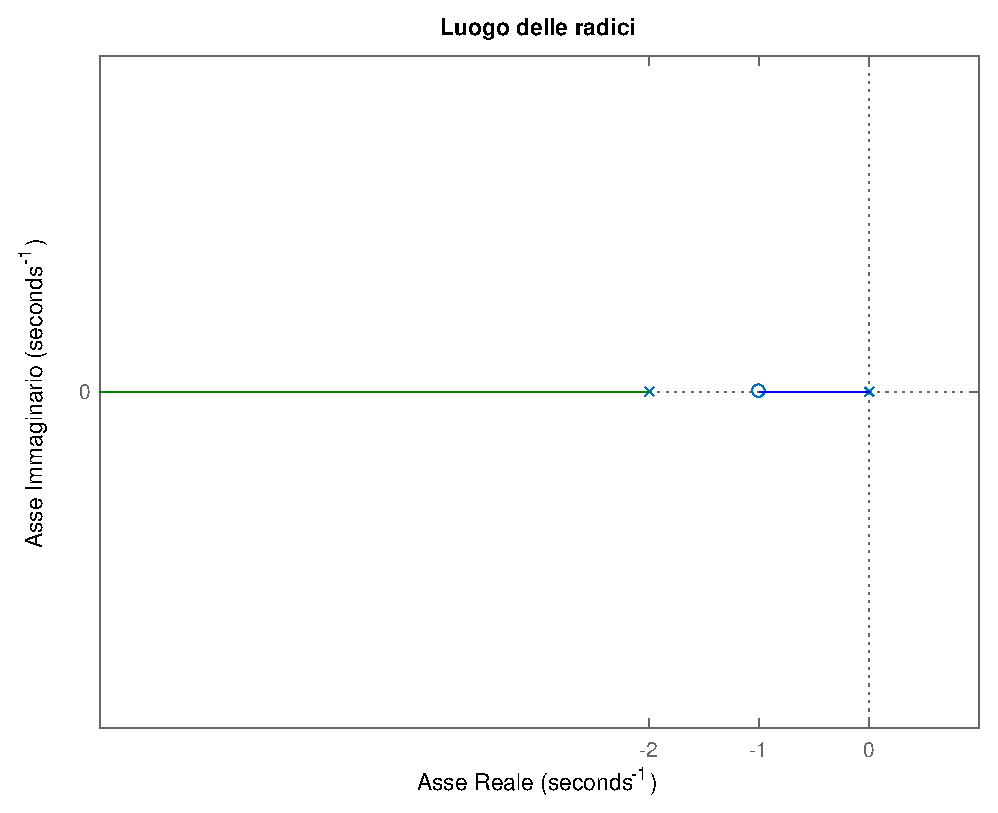
\includegraphics[scale=.6]{mod1/assets/rl_ex31}
\end{figure}

\begin{itemize}
	\item \emph{Punti di singolarità}:
		\begin{itemize}
			\item poli: \(\bigl\{-2, 0\bigr\}\)
			\item zeri: \(\bigl\{-1\bigr\}\)
		\end{itemize}
	\item \emph{Asintoti}:
		Determino centroide e angolo di inclinazione degli asintoti
		\[
			\sigma_a = \frac{0 -2 +1}{1} = -1
			\qquad
			\theta_a = \frac{\Bigl(2\cdot\bigl[0\bigr]+1\Bigr)\pi}{1} = \pi
		\]
	\item L'esercizio non richiede altro lavoro perché non presenta punti doppi,
		di intersezione con l'asse immaginario, etc.
	\item \emph{Stabilità}:
		\[\begin{cases}
			k = 0 & \text{sistema \emph{semplicemente stabile}} \\
			k > 0 & \text{sistema \emph{asintoticamente stabile}} \\
		\end{cases}\]
\end{itemize}


\subsection{Esercizio}
Sia data la seguente funzione di trasferimento:
\[
	G(s) = \frac{s+1}{s^2}
\]
Determinare il luogo delle radici al variare di \(k > 0\).

\paragraph{Soluzione}

\begin{figure}[ht]
	\centering
	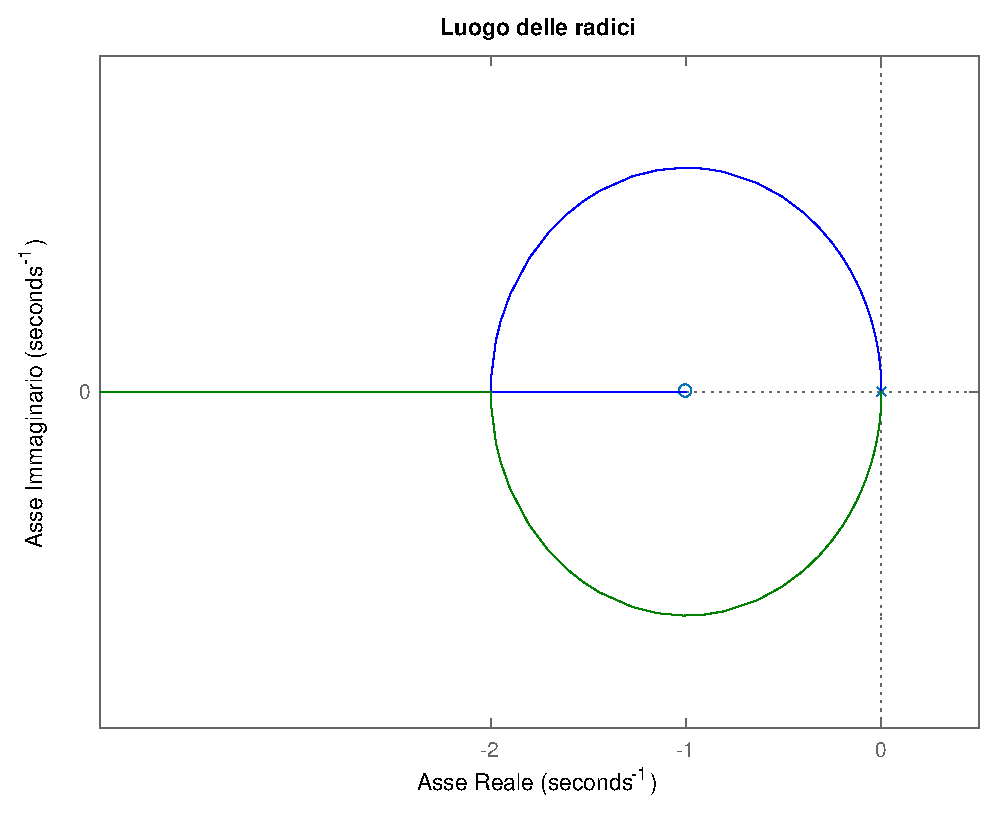
\includegraphics[scale=.6]{mod1/assets/rl_ex32}
\end{figure}

\begin{itemize}
	\item \emph{Punti di singolarità}:
		\begin{itemize}
			\item poli: \(\bigl\{ 0\,[\times 2] \bigr\}\)
			\item zeri: \(\bigl\{ -1 \bigr\}\)
		\end{itemize}
	\item \emph{Asintoti}:
		\[
			\sigma_a = \frac{0+1}{1} = 1 \qquad
			\theta_a = \frac{\Bigl(2\cdot\bigl[0\bigr]+1\Bigr)\pi}{1} = \pi
		\]
	\item Gli angoli di arrivo e di partenza sono entrambi di
		\(\pm \frac{\pi}{2}\), questo perché non sono punti complessi e
		coniugati.
	\item Posizione del punto di confluenza:
		\[
			G^\prime(s) = \frac{s^2 -2s(s+1)}{\cancel{s^2}} = 0
			\rightarrow s(s+2) = 0
			\implies s= \begin{cases} 0 \\ \bm{-2} \end{cases}
		\]
	\item Stabilità:
		\[\begin{cases}
			\text{Se } k = 0\colon & \text{sistema \emph{semplicemente stabile}} \\
			\text{Se } k > 0\colon & \text{sistema \emph{asintoticamente stabile}}
		\end{cases}\]
\end{itemize}


\subsection{Esercizio}
Sia data la seguente funzione di trasferimento
\[
	G(s) = \frac{1}{s(s+1)(s+5)}
\]
Determinare il luogo delle radici al variare di \(k>0\).

\paragraph{Soluzione}

\begin{figure}[ht]
	\centering
	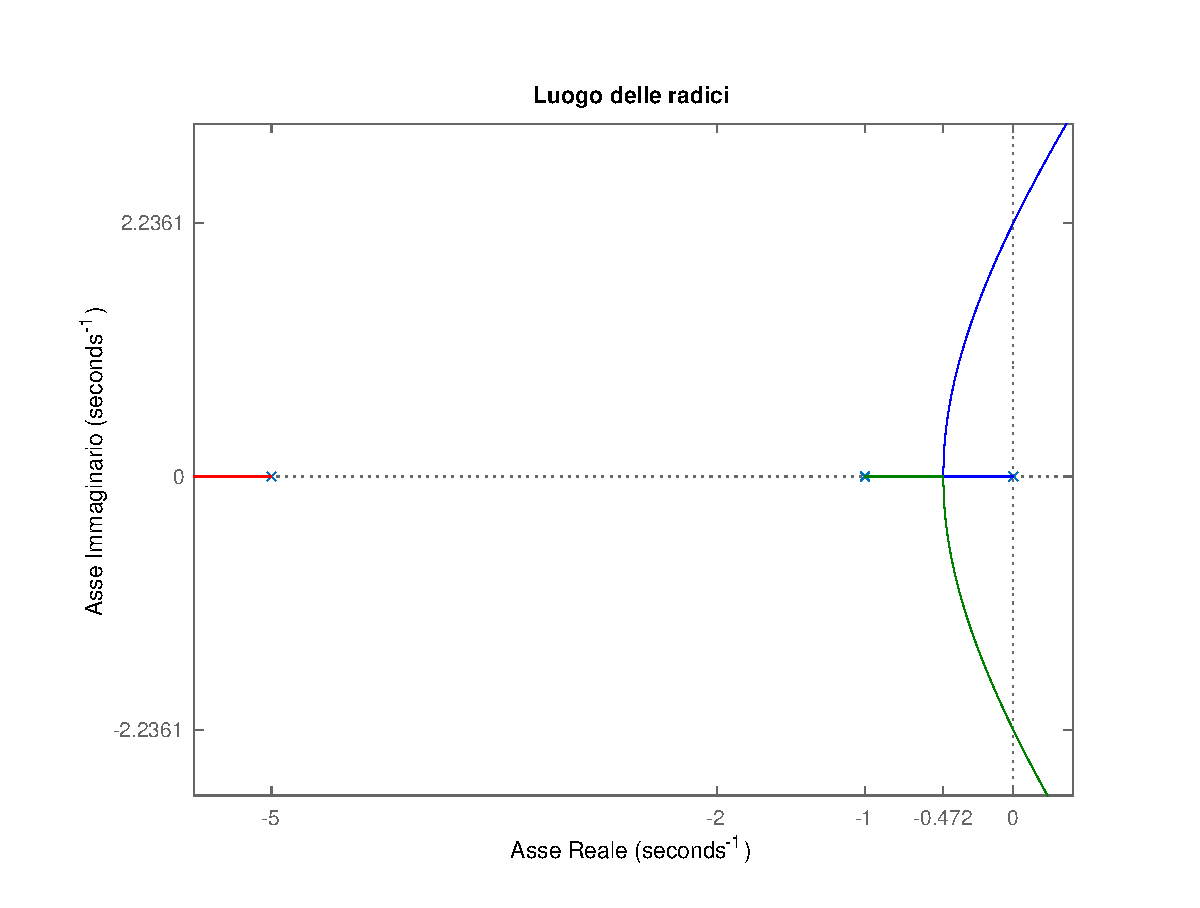
\includegraphics[scale=.6]{mod1/assets/rl_ex33}
\end{figure}

\begin{itemize}
	\item \emph{Punti di singolarità}:
		\begin{itemize}
			\item poli: \(\bigl\{ -5, -1, 0 \bigr\}\)
		\end{itemize}
	\item \emph{Asintoti}:
		\begin{align*}
			& \sigma_a = \frac{0-1-5}{3} = -2 \\
			& \theta_a = \frac{\Bigl( 2 \cdot \bigl[ 0, \dots, 2 \bigr] +1 \Bigr) \pi}{3} = \Bigl[ \frac{\pi}{3}, \pi, \frac{5}{3}\pi \Bigr]
		\end{align*}
	\item \emph{Punto doppio di emergenza}:
		\[
			G^\prime (s) = 0 \rightarrow -3s^2 -12s -5=0 \rightarrow s_{1,2} = \frac{-6\pm\sqrt{21}}{3} = \begin{cases} \bm{-0.472} \\ -3.527 \end{cases}
		\]
		Si sceglie il primo perché è il valore che appartiene al luogo delle radici.
	\item \emph{Punti di intersezione con l'asse immaginario}:
		applico il criterio di Routh per \(P(s) = s^3 +6s +5s +k\):
		\[\begin{array}{r|rr}
			s^3      & 1 & 5 \\
			\bm{s^2} & 6 & k \\
			s^1      & \bm{30-k} \\
			s^0      & k
		\end{array}\]
		\[
			k = 30 \rightarrow 6s^2+30 = 0 \rightarrow s = \pm \jmath \sqrt{5}
		\]
	\item \emph{Stabilità}:
		\[\begin{cases}
			\text{Se } k = 0\colon & \text{sistema \emph{semplicemente stabile}} \\
			\text{Se } 0 < k < 30\colon & \text{sistema \emph{asintoticamente stabile}} \\
			\text{Se } k = 30\colon & \text{sistema \emph{semplicemente stabile}} \\
			\text{Se } k > 30\colon & \text{sistema \emph{instabile} con 2 poli instabili}
		\end{cases}\]
\end{itemize}


\subsection{Esercizio}
Sia data la seguente funzione di trasferimento:
\[
	G(s) = \frac{(s+1.5)(s+4)}{s(s+1)(s+2.5)}
\]
Determinare il luogo delle radici per \(k>0\).

\paragraph{Soluzione}

\begin{figure}[ht]
	\centering
	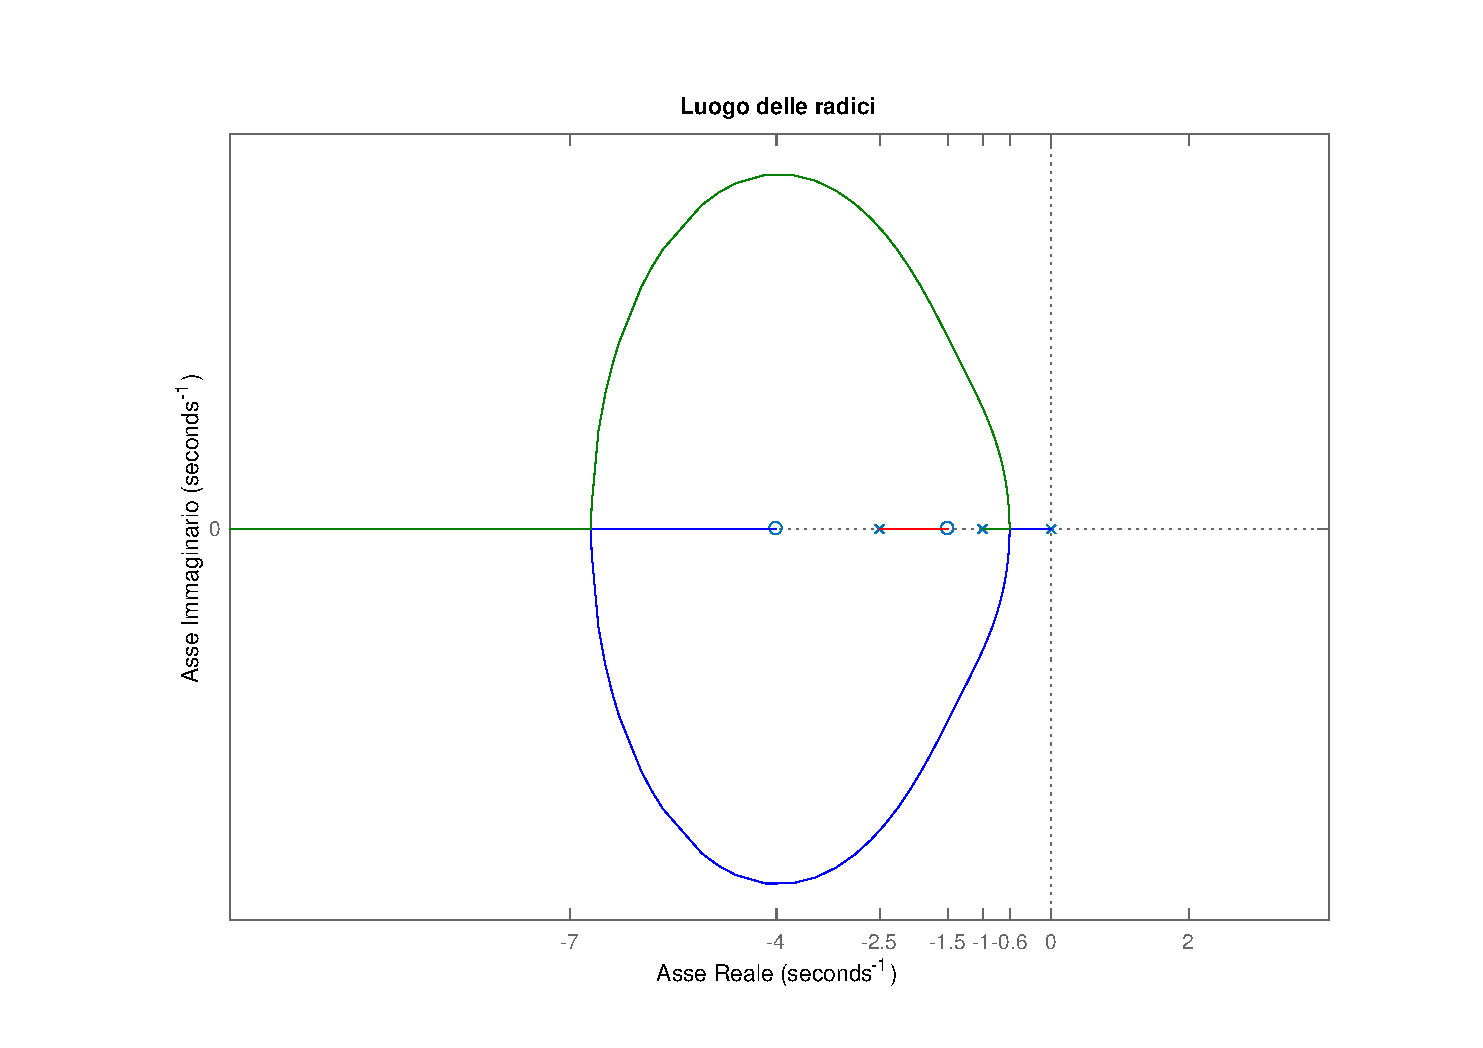
\includegraphics[scale=.6]{mod1/assets/rl_ex34}
\end{figure}

\begin{itemize}
	\item \emph{Punti di singolarità}:
		\begin{itemize}
			\item poli: \(\bigl\{ -2.5, -1, 0 \bigr\}\)
			\item zeri: \(\bigl\{ -4, -1.5 \bigr\}\)
		\end{itemize}
	\item \emph{Asintoti}:
		\begin{align*}
			& \sigma_a = \frac{0-1-2.5+1.5+4}{1} = 2 \\
			& \theta_a = \frac{\Bigl( 2 \cdot \bigl[0\bigr] +1 \Bigl)}{1} = \pi
		\end{align*}
	\item \emph{Punto doppio di emergenza}:
		lo ricavo con la tabella di taratura
		\[\begin{array}{rr}
			\toprule
			s & k \\
			\midrule
			-0.2 & 0.074 \\
			-0.4 & 0.127 \\
			\bm{-0.6} & \bm{0.149} \\
			-0.8 & 0.12 \\
			\bottomrule
		\end{array}\]
		Per \(s = -0.6\) si ha il massimo locale, ovvero il punto più
		approssimato al punto di emergenza.
	\item \emph{Punto doppio di confluenza}:
		\[\begin{array}{rr}
			\toprule
			s & k \\
			\midrule
			-5 & 14.286 \\
			-6 & 11.667 \\
			\bm{-7} & \bm{11.454} \\
			-8 & 11.846 \\
			\bottomrule
		\end{array}\]
		Per \(s = -7\) si ha il minimo locale, ovvero il più approssimato
		al punto di confluenza.
	\item \emph{Stabilità}:
		\[\begin{cases}
			k = 0\colon & \text{sistema \emph{semplicemente stabile}} \\
			k > 0\colon & \text{sistema \emph{asintoticamente stabile}}
		\end{cases}\]
\end{itemize}


\subsection{Esercizio}
Sia data la seguente funzione di trasferimento:
\[
	G(s) = \frac{s+1}{s^2 (s+4)}
\]
Determinare il luogo delle radici per \(k>0\).

\paragraph{Soluzione}

\begin{figure}[ht]
	\centering
	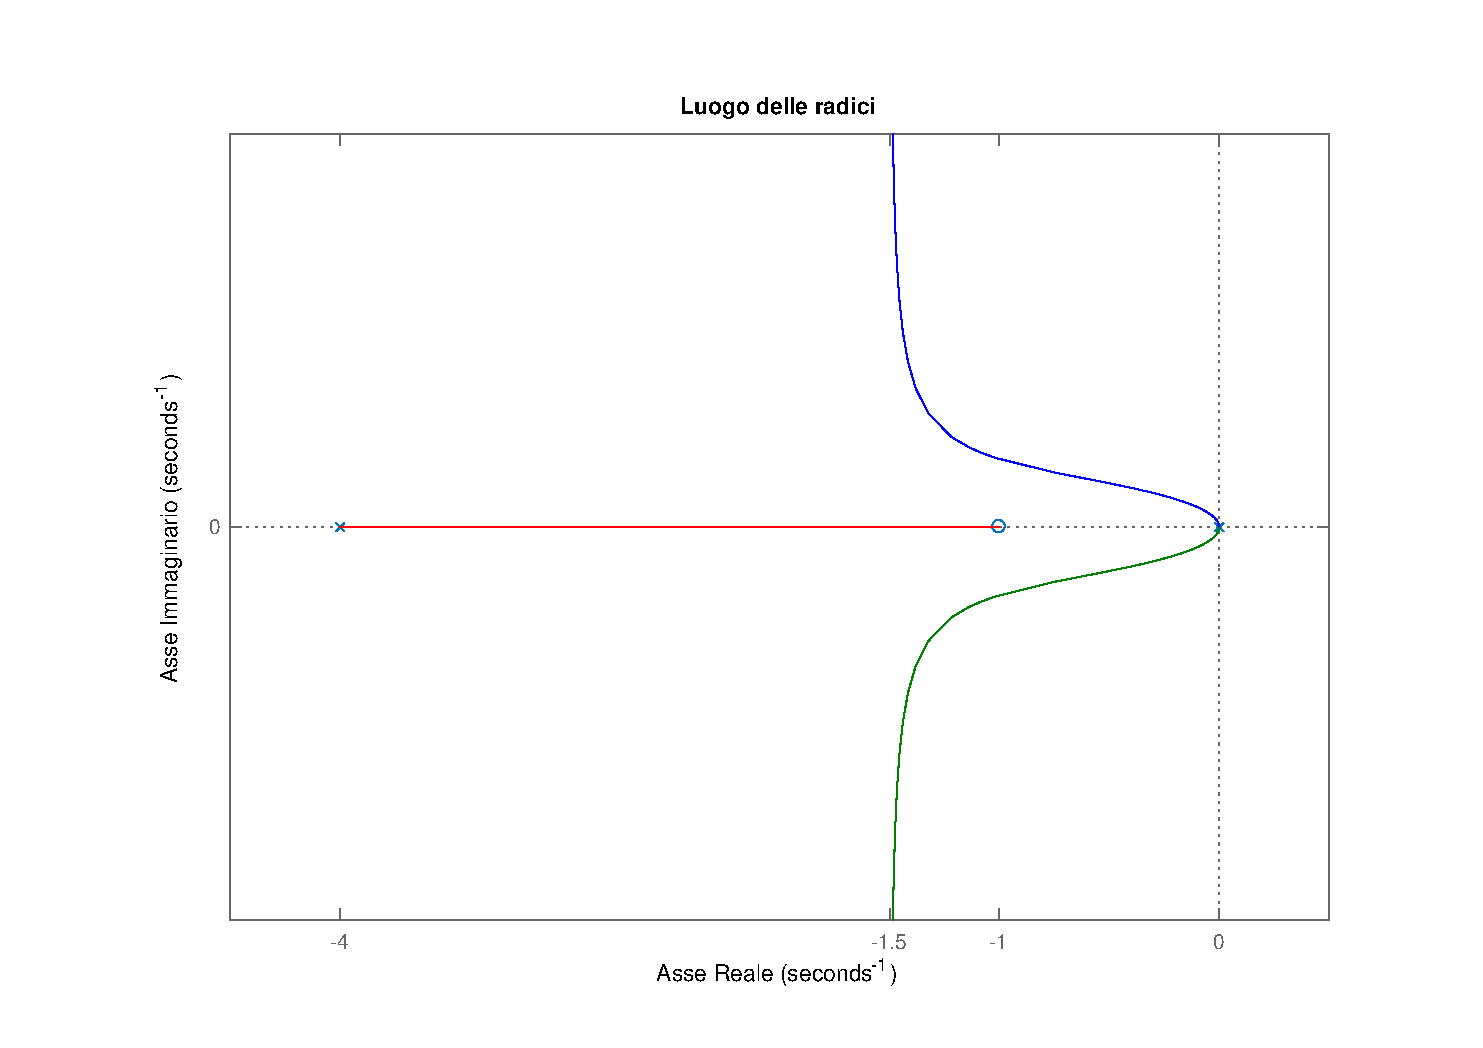
\includegraphics[scale=.6]{mod1/assets/rl_ex35}
\end{figure}

\begin{itemize}
	\item \emph{Punti di singolarità}:
		\begin{itemize}
			\item poli: \(\bigl\{ -4, 0\,[\times 2] \bigr\}\)
			\item zeri: \(\bigl\{ -1 \bigr\}\)
		\end{itemize}
	\item \emph{Asintoti}:
		\begin{align*}
			& \sigma_a = \frac{0-4+1}{2} = -\frac{3}{2} \\
			& \theta_a = \frac{\Bigl( 2 \cdot \bigl[ 0,1 \bigr] \pi \Bigr) \pi}{2} = \Bigl[ \frac{\pi}{2}, \frac{3}{2}\pi \Bigr]
		\end{align*}
	\item \emph{Angoli di partenza dei rami}: \(\frac{\pi}{2}\)
\end{itemize}


\subsection{Esercizio}
Sia data la seguente funzione di trasferimento
\[
	G(s) = \frac{s+1}{s^2 (s+9)}
\]
Determinare il luogo delle radici per \(k>0\).

\paragraph{Soluzione}

\begin{figure}[ht]
	\centering
	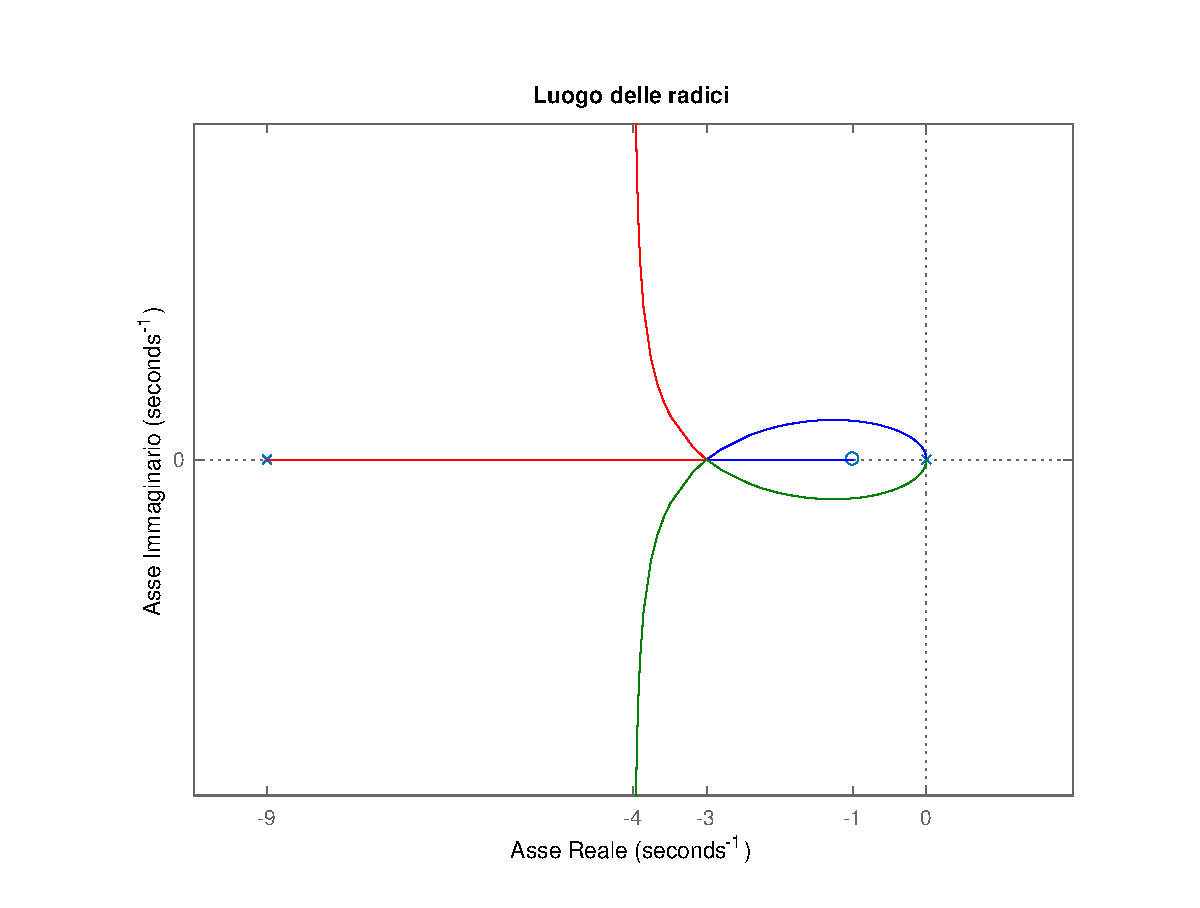
\includegraphics[scale=.6]{mod1/assets/rl_ex36}
\end{figure}

\begin{itemize}
	\item \emph{Punti di singolarità}:
		\begin{itemize}
			\item poli: \(\bigl\{ -9, 0\,[\times 2] \bigr\}\)
			\item zeri: \(\bigl\{ -1 \bigr\}\)
		\end{itemize}
	\item \emph{Asintoti}:
		\begin{align*}
			& \sigma_a = \frac{0-9+1}{2} = -4 \\
			& \theta_a = \frac{\Bigl(2 \cdot \bigl[ 0,1 \bigr] +1\Bigr) \pi}{2} = \Bigl[ \frac{\pi}{2}, \frac{3}{2}\pi \Bigr]
		\end{align*}
\end{itemize}
I poli all'origine si dirigono verso gli asintoti, ma sono soggetti all'attrazione
dello zero; quindi verifico possibili punti tripli nell'intervallo \((-4,-1)\):
\[
	G^\prime(s) = \frac{s^2(s+9) -\bigl(2s(s+9)+s^2\bigr)(s+1)}{\cancel{s^4 (s+9)^2}} = 0
	\rightarrow s(s+3)^2 = 0 \rightarrow s = \begin{cases} 0 \\ \bm{-3} \end{cases}
\]
Quindi si ha effettivamente un punto triplo in \(s = -3\), che impone la convergenza
dei rami che partono dai due poli all'origine e la loro emergenza verso gli asintoti.


\subsection{Esercizio}
Sia data la seguente funzione di trasferimento:
\[
	G(s) = \frac{1}{s(s+2)\bigl( (s+1)^2 +4 \bigr)}
\]
Determinare il luogo delle radici per \(k>0\).

\paragraph{Soluzione}

\begin{figure}[ht]
	\centering
	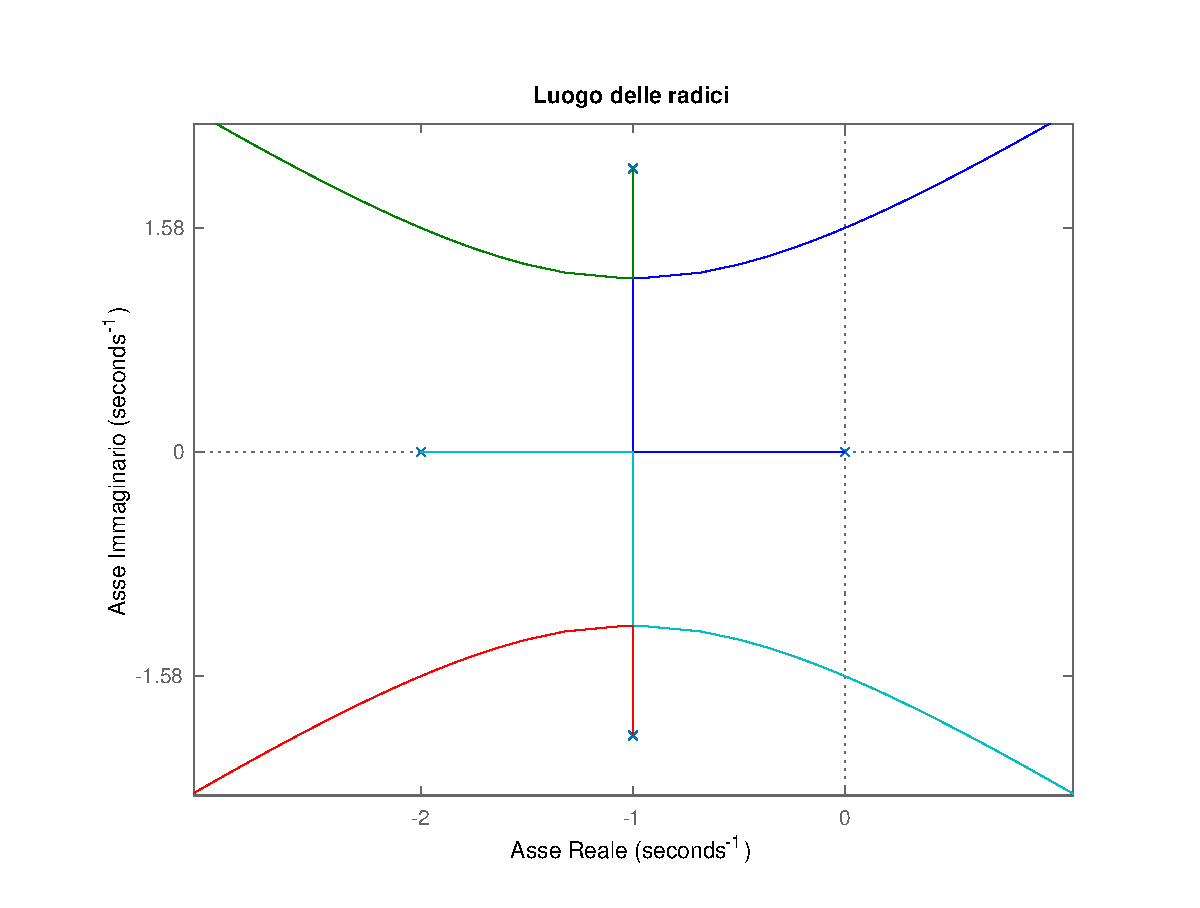
\includegraphics[scale=.6]{mod1/assets/rl_ex37}
\end{figure}

\begin{itemize}
	\item \emph{Punti di singolarità}:
		\begin{itemize}
			\item poli: \(\bigl\{ -2, -1\pm\jmath2, 0 \bigr\}\)
		\end{itemize}
	\item \emph{Asintoti}:
		\begin{align*}
			& \sigma_a = \frac{0-2-2(1\cancel{\pm\jmath2})}{4} = -1 \\
			& \theta_a = \frac{\Bigl(2 \cdot \bigl\{ 0,1,2,3 \bigr\} +1)\pi}{4} = \Bigl\{ \frac{\pi}{4}, \frac{3}{4}\pi, \frac{5}{4}\pi, \frac{7}{4}\pi \Bigr\}
		\end{align*}
	\item \emph{Punti doppi}:
		calcolando \(G^\prime(s) = 0\) si ottiene l'equazione
		\[
			2s^3 +6s^2 +9s +5 = 0 \rightarrow s = \begin{cases} -1 \\ -1 \pm\jmath\sqrt{\frac{3}{2}} \end{cases}
		\]
		Questo significa che ci sono 3 punti doppi dove i poli si
		''scontrano'' e così si diramano.
	\item \emph{Angoli di partenza} per i poli complessi e coniugati:
		\begin{align*}
			\varphi_+ &= \pi - \angle(-1+\jmath2) -\angle(-1+\jmath2+2) -\angle(\cancel{-1}+\jmath2\cancel{+1}+\jmath2) = \\
				  &= \pi +\arctan{2} -\pi -\arctan{2} -\frac{\pi}{2} = -\frac{\pi}{2} \\
			\varphi_- &= \pi -\angle(-1-\jmath2) -\angle(-1-\jmath2+2) -\angle(\cancel{-1}-\jmath2\cancel{+1}-\jmath2) = \\
				  &= \pi +\arctan{2} -\pi -\arctan{2} +\frac{\pi}{2} = \frac{\pi}{2}
		\end{align*}
	\item \emph{Intersezioni con l'asse immaginario}:
		\[
			P(s) = s^4 +4s^3 +9s^2 +10s +k
		\]
		\[
			\begin{array}{r|rrr}
				s^4 & 1 &  9 & k \\
				s^3 & 4 & 10 \\
				\bm{s^2} & \cancelto{13}{26} & \cancelto{2}{4} k \\
				s^1 & \bm{65-4k} \\
				s^0 & 2k
			\end{array}
		\]
		Per \(k = \frac{65}{4} = \frac{13\cdot5}{4} \rightarrow \cancel{13}s^2 + \frac{\cancel{13}\cdot5}{2} = 0 \rightarrow s = \pm\jmath\sqrt{\frac{5}{2}}\)
	\item \emph{Stabilità}:
		\[\begin{cases}
			k=0\colon & \text{sistema \emph{semplicemente stabile}} \\
			0<k<\frac{13}{2}\colon & \text{sistema \emph{asintoticamente stabile}} \\
			k=\frac{13}{2}\colon & \text{sistema \emph{semplicemente stabile}} \\
			k>\frac{13}{2}\colon & \text{sistema \emph{instabile} con 2 poli instabili}
		\end{cases}\]
\end{itemize}


\subsection{Esercizio}
Sia data la seguente funzione di trasferimento:
\[
	G(s) = \frac{1}{s(s+1)(s+3)(s+4)}
\]
Determinare il luogo delle radici per \(k>0\) e \(k<0\).

\paragraph{Soluzione per \(k > 0\)}

\begin{figure}[ht]
	\centering
	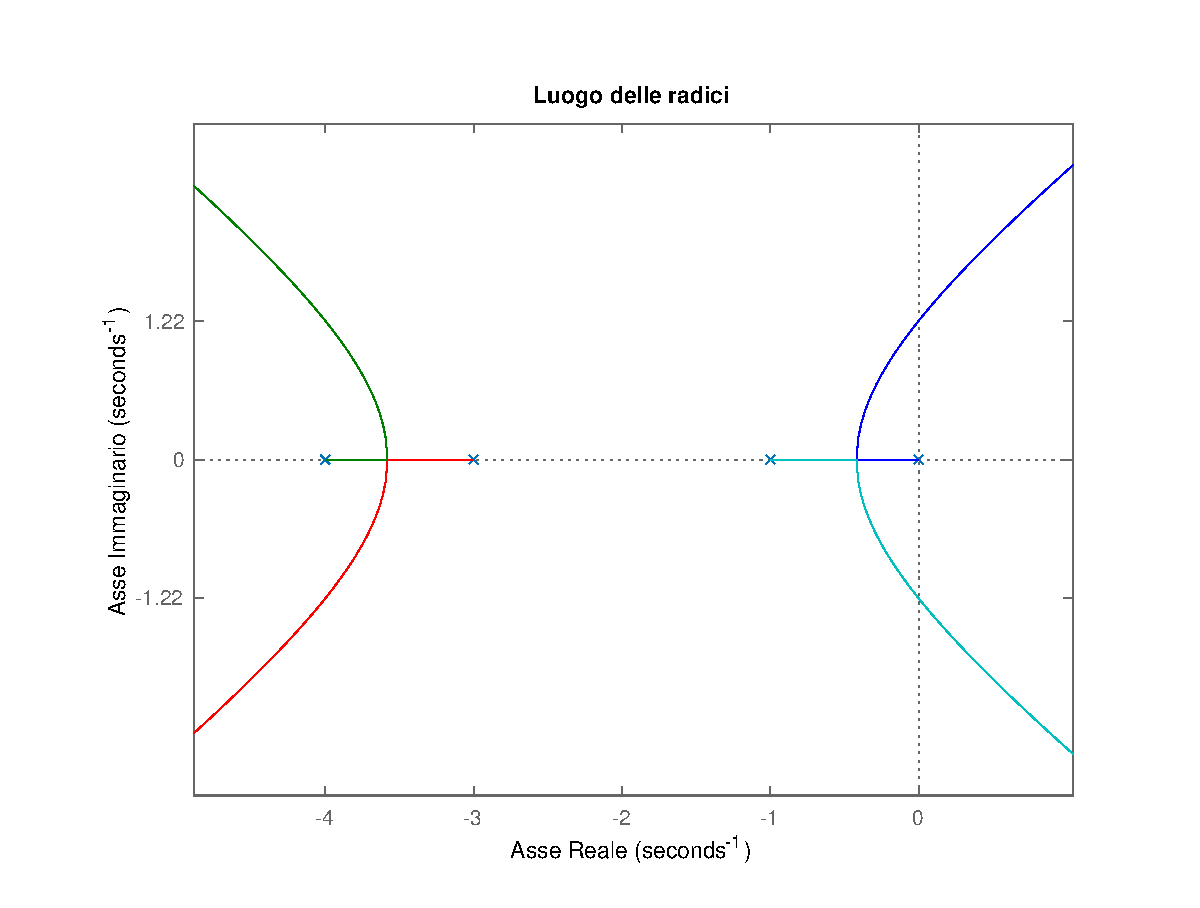
\includegraphics[scale=.6]{mod1/assets/rl_ex38}
\end{figure}

\begin{itemize}
	\item \emph{Punti di singolarità}:
		\begin{itemize}
			\item poli: \(\bigl\{ -4,-3,-1,0 \bigr\}\)
		\end{itemize}
	\item \emph{Asintoti}:
		\begin{align*}
			& \sigma_a = \frac{0-1-3-4}{4} = -2 \\
			& \theta_a = \frac{\Bigl(2\cdot\bigl[0,1,2,3\bigr]+1\Bigr)\pi}{4} = \Bigl[ \frac{\pi}{4},\frac{3}{4}\pi,\frac{5}{4}\pi,\frac{7}{4}\pi \Bigr]
		\end{align*}
	\item \emph{Punti doppi}: \(k = -s(s+1)(s+3)(s+4)\)
		\[\begin{array}{rr}
			\toprule
			s 	  & k 		\\
			\midrule
			-0.3 	  & 2.098 	\\
			\bm{-0.5} & \bm{2.187}	\\
			-0.7 	  & 1.594	\\
			\bottomrule
		\end{array}\]
		\(s=-0.5\) è un punto doppio di emergenza.
		\[\begin{array}{rr}
			\toprule
			s 	  & k 		\\
			\midrule
			-3.3 	  & 1.594 	\\
			\bm{-3.5} & \bm{2.187} 	\\
			-3.7 	  & 2.098 	\\
			\bottomrule
		\end{array}\]
		\(s=-3.5\) è un punto doppio di emergenza.
	\item \emph{Intersezioni con l'asse immaginario}:
		\[
			P(s) = s^4 +8s^3 +19s^2 +12s +k
		\]
		\[\begin{array}{r|rrr}
			s^4 	 &  1 & 19 & k  \\
			s^3 	 &  8 & 12 	\\
			\bm{s^2} & 35 & 2k 	\\
			s^1 	 & \bm{105-4k} 	\\
			s^0 	 & 2k
		\end{array}\]
		\(k = \frac{105}{4} = \frac{35\cdot3}{4} \rightarrow s^2+\frac{3}{2} = 0 \rightarrow s = \pm\jmath\sqrt{\frac{3}{2}}\)
	\item \emph{Stabilità}:
		\[\begin{cases}
			k = 0\colon & \text{sistema \emph{semplicemente stabile}} \\
			0<k<\frac{105}{4}\colon & \text{sistema \emph{asintoticamente stabile}} \\
			k = \frac{105}{4}\colon & \text{sistema \emph{semplicemente stabile}} \\
			k > \frac{105}{4}\colon & \text{sistema \emph{instabile} con 2 poli instabili}
		\end{cases}\]
\end{itemize}

\paragraph{Soluzione per \(k < 0\)}

\begin{figure}[ht]
	\centering
	\includegraphics[scale=.6]{mod1/assets/rl_ex38n}
\end{figure}

\begin{itemize}
	\item \emph{Asintoti}:
		\[
			\sigma_a = -2 \qquad \theta_a = \frac{2\cdot\bigl[ 0,1,2,3 \bigr]\pi}{4} = \Bigl[ 0,\frac{\pi}{2},\pi,\frac{3}{2}\pi \Bigr]
		\]
	\item \emph{Stabilità}: per \(k < 0\) il sistema è \emph{instabile} con 1 polo instabile.
\end{itemize}

\paragraph{Determinare i poli per i punti critici}
\[\begin{cases}
	k = 0\colon & \bigl\{ -4,-3,-1,0 \bigr\} \\
	k = \frac{105}{4}\colon & \begin{cases}
		\text{2 poli puramente immaginari: } s_{1,2} = \pm\jmath\sqrt{\frac{3}{2}} \\
		\text{2 poli stabili: } s_{3,4} = -4 \pm\jmath\sqrt{\frac{3}{2}}
	\end{cases}
\end{cases}\]


\subsection{Esercizio}
Sia data la seguente funzione di trasferimento:
\[
	G(s) = \frac{s-1}{(s+2)(s-2)(s+4)}
\]
Determinare il luogo delle radici per \(k\in\mathbb{R}^2\).

\paragraph{Soluzione}

\begin{figure}[ht]
	\centering
	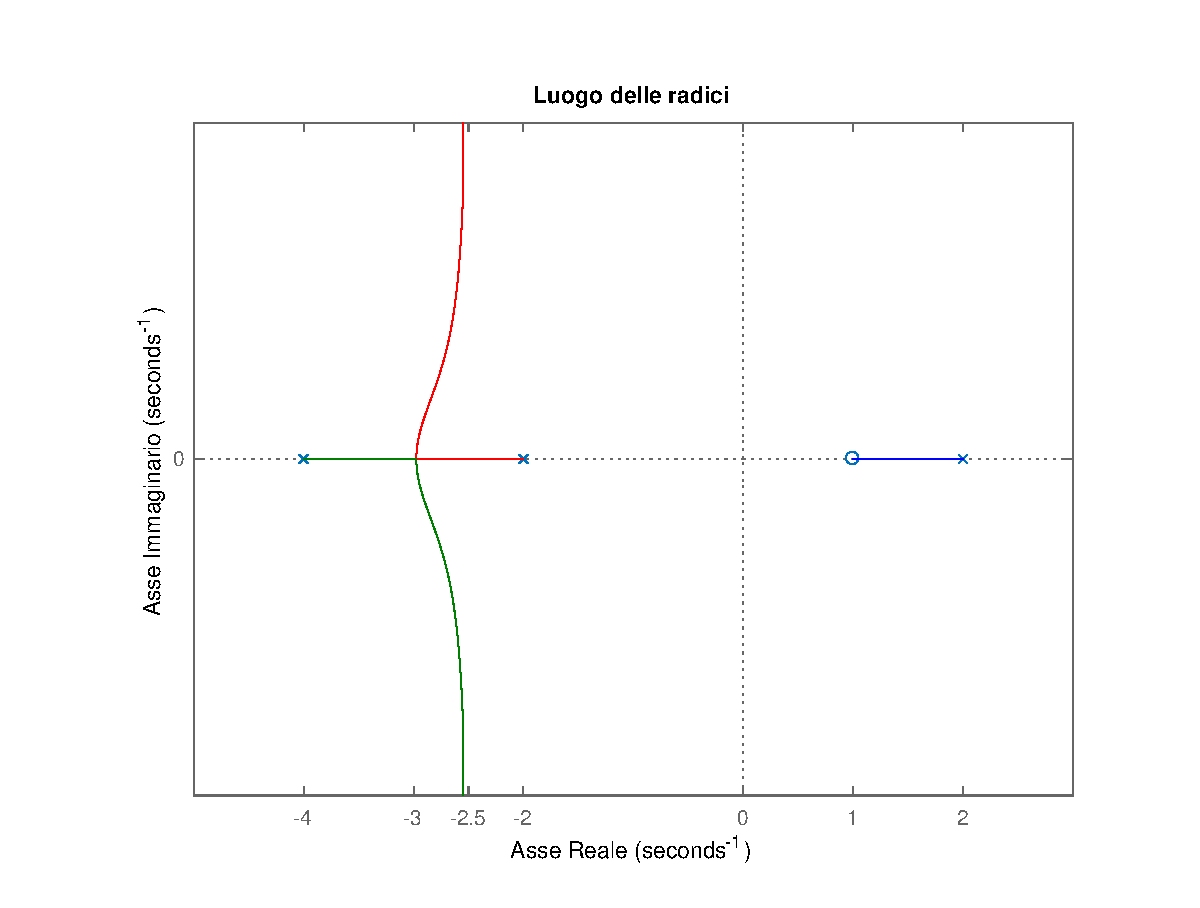
\includegraphics[scale=.6]{mod1/assets/rl_ex39}
\end{figure}

\begin{itemize}
	\item \emph{Punti di singolarità}:
		\begin{itemize}
			\item poli: \(\bigl\{ -4,-2,2 \bigr\}\) \\
			\item zeri: \(\bigl\{ 1 \bigr\}\)
		\end{itemize}
	\item \emph{Asintoti}:
		\[
			\sigma_a = \frac{-2+2-4-1}{2} = -\frac{5}{2} \qquad
			\theta_a = \frac{\Bigl(2\cdot \bigl[0,1\bigr] +1\Bigr)\pi}{2} = \Bigl[ \frac{\pi}{2},\frac{3}{2}\pi \Bigr]
		\]
	\item \emph{Punti doppi}:
		\[
			k = -\frac{1}{G(s)} = + \frac{(s+2)(s-2)(s+4)}{1-s} \quad
			\text{per } s \in \Bigl(-4,-\frac{5}{2}\Bigr)
		\]
		\[\begin{array}{rr}
			\toprule
			s 	  & k 		\\
			\midrule
			-3.5 	  & 0.917 	\\
			-3.3 	  & 1.123 	\\
			\bm{-3.0} & \bm{1.25} 	\\
			-2.7 	  & 1.156	\\
			\bottomrule
		\end{array}\]
		Per \(s=-3\) si ha un punto doppio di emergenza.
	\item \emph{Stabilità}: il sistema è sempre \emph{instabile} con 1 polo instabile.
\end{itemize}


\subsection{Esercizio}
Siano dati
\[
	G_p(s) = \frac{s+1}{s(s-5)(s+5)} \qquad G_c(s) = k
\]
Determinare il luogo delle radici del sistema ad anello chiuso per \(k>0\).

\paragraph{Soluzione}

Si ricorda che
\begin{center}\begin{tikzpicture}[auto,node distance=2cm,>=latex']
	\node [input] (x) {};
	\node [sum, right of=x] (sum) {};
	\node [block, right of=sum] (B) {\(G_c(s)\)};
	\node [block, right of=B] (D) {\(G_p(s)\)};
	\node [tmp, right of=D] (tmp) {};
	\node [output, right of=tmp] (y) {};
	\draw [->] (x) -- node[pos=0]{\(x\)} (sum);
	\draw [->] (sum) -- (B) -- node[pos=0.5,name=achr]{} (D) -- (tmp) -- node[pos=1]{\(y\)} (y);
	\node [block, below of=achr, node distance=1.5cm] (C) {\(H(s)\)};
	\draw [->] (tmp) |- (C) -| node[pos=0.9,anchor=west]{\(-\)} (sum);
\end{tikzpicture}\end{center}
Quindi si ha \(G(s)H(s) = G(s)\) considerando \(H(s)\) unitario.

\begin{figure}[ht]
	\centering
	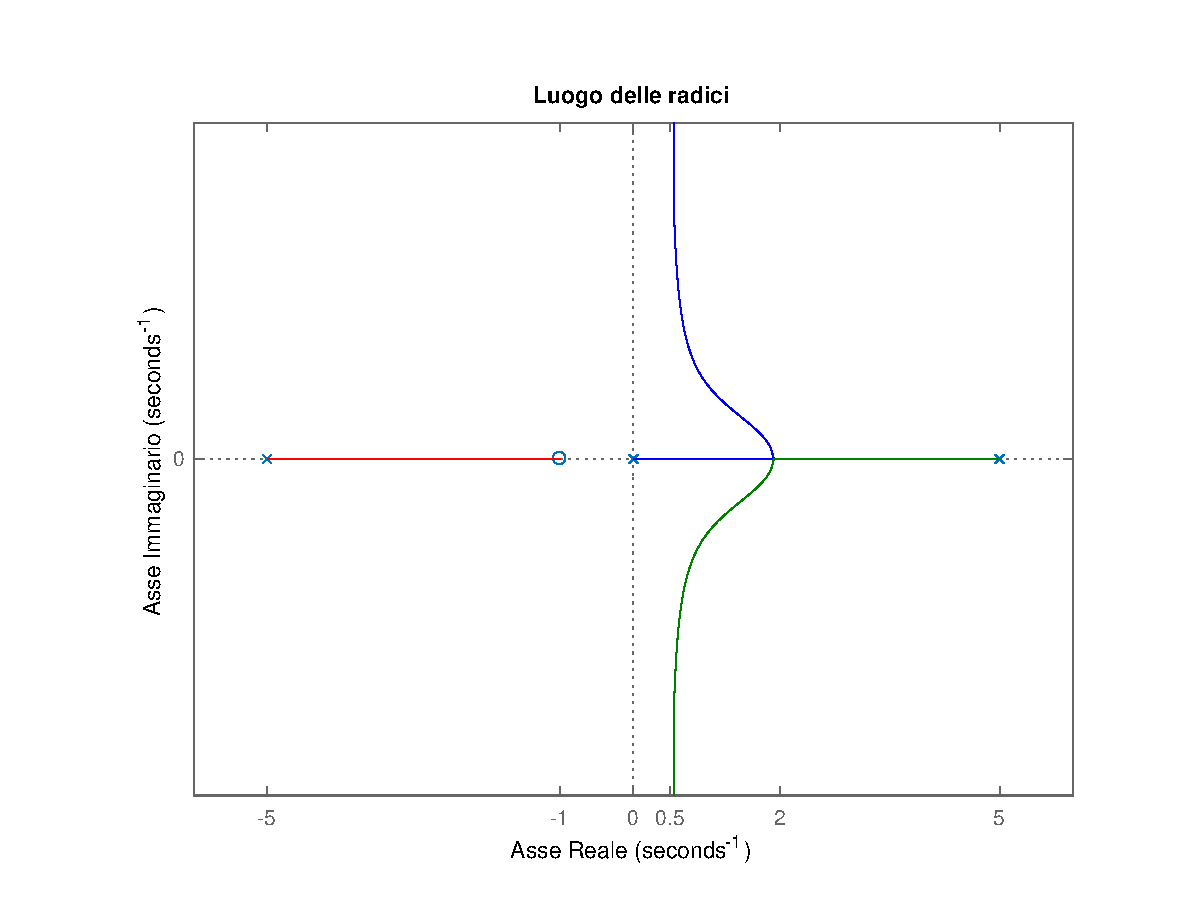
\includegraphics[scale=.6]{mod1/assets/rl_ex310}
\end{figure}

\begin{itemize}
	\item \emph{Punti di singolarità}:
		\begin{itemize}
			\item poli: \(\bigl\{ -1 \bigr\}\)
			\item zeri: \(\bigl\{ -5,0,5 \bigr\}\)
		\end{itemize}
	\item \emph{Asintoti}:
		\[
			\sigma_a = \frac{0+5-5+1}{2} = \frac{1}{2} \qquad
			\theta_a = \frac{\Bigl(2\cdot \bigl[0,1\bigr]\Bigr)\pi}{2} = \Bigl[ \frac{\pi}{2},\frac{3}{2}\pi \Bigr]
		\]
	\item \emph{Punti doppi}:
		\[
			k = -\frac{1}{G(s)} = -\frac{s(s-5)(s+5)}{s+1} \quad
			\text{per } s \in \Bigl( \frac{1}{2},5 \Bigr)
		\]
		\[\begin{array}{rr}
			\toprule
			s 	&       k \\
			\midrule
			1 	&      12 \\
			1.5 	&   13.65 \\
			\bm{2} 	& \bm{14} \\
			2.5 	&   13.39 \\
			\bottomrule
		\end{array}\]
		Per \(s=-2\) si ha un punto doppio di emergenza.
	\item \emph{Stabilità}: per \(k \geq 0\) il sistema è \emph{instabile}
		con 2 poli instabili.
\end{itemize}


\subsection{Esercizio}
Sia data la seguente funzione di trasferimento:
\[
	G(s) = \frac{s-1}{s^2(s^2+4s+8)}
\]
Determinare il luogo delle radici per \(k>0\) e \(k<0\).

\paragraph{Soluzione per \(k>0\)}
È possibile semplificare \(G(s)\) per rendere noti i poli coniugati e complessi:
\[
	G(s) = \frac{s-1}{s^2\bigl( (s+2)^2 +4 \bigr)}
\]

\begin{figure}[ht]
	\centering
	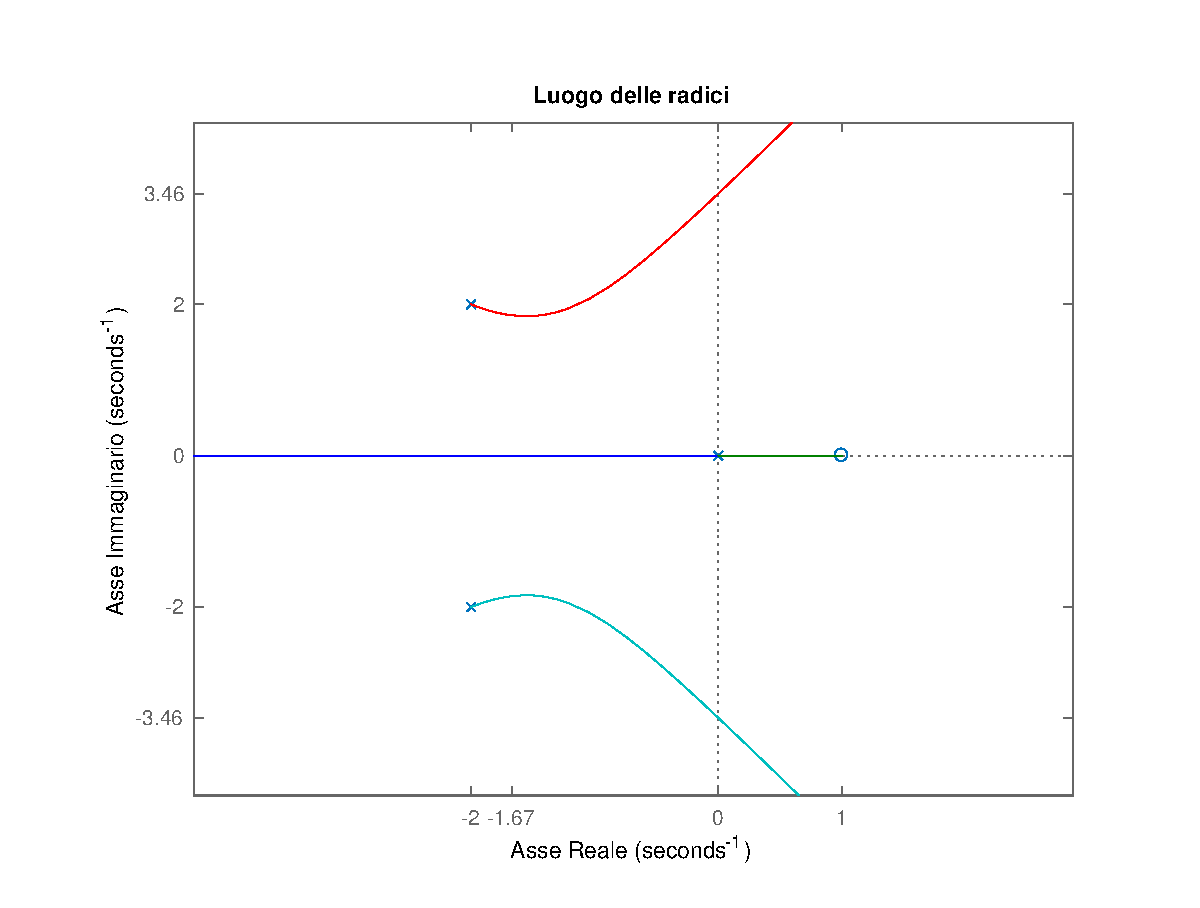
\includegraphics[scale=.5]{mod1/assets/rl_ex311}
	\caption{per \(k>0\)}
\end{figure}

\begin{itemize}
	\item \emph{Punti di singolarità}:
		\begin{itemize}
			\item poli: \(\bigl\{ -2\pm\jmath2, 0\,[\times 2] \bigr\}\)
			\item zeri: \(\bigl\{ 1 \bigr\}\)
		\end{itemize}
	\item \emph{Asintoti}:
		\[
			\sigma_a = \frac{0-4\pm\jmath2-1}{3} = -\frac{5}{3} \qquad
			\theta_a = \frac{\Bigl(2\cdot \bigl[ 0,1,2 \bigr] +1 \Bigr)\pi}{3} = \Bigl[ \frac{\pi}{3},\pi,\frac{5}{3}\pi \Bigr]
		\]
	\item \emph{Intersezioni con l'asse immaginario}:
		\[
			P(s) = s^4 +4s^3 +8s^2 +ks -k
		\]
		\[\begin{array}{r|rrr}
			s^4 	 & 1    &   8 & -k \\
			s^3 	 & 4    &   k 	   \\
			\bm{s^2} & 32-k & -4k 	   \\
			s^1 	 & \bm{48-k} 	   \\
			s^0 	 & -4k
		\end{array}\]
		Per \(k = 48 = 16\cdot3\) si ha \(-16s^2-16\cdot12=0 \rightarrow
		s = \pm\jmath2\sqrt{3}\).
	\item \emph{Angoli di partenza} per \(s = \pm\jmath2\sqrt{3}\):
		\begin{align*}
			\varphi_- &= \pi + \angle(-2-\jmath2-1) -\angle(-2-\jmath2+2-\jmath2) -2\angle(-2-\jmath2-0) = \\
				  &= \pi + \arctan{\frac{2}{3}} -\pi +\frac{\pi}{2} -2\arctan{1} +2\pi = \\
				  &= 2\pi +0.588 +\frac{\pi}{2} -2\frac{\pi}{4} = \SI{0.588}{\radian} \\
			\varphi_+ &= \pi +\angle(-2+\jmath2-1) -\angle(-2+\jmath2+2+\jmath2) -2\angle(-2+\jmath2-0) = \\
				  &= \pi +\arctan{-\frac{2}{3}} +\pi -\frac{\pi}{2} -2\arctan{-1} -2\pi = \\
				  &= -0.588 -\frac{\pi}{2} -2\frac{\pi}{4} = \SI{-0.588}{\radian}
		\end{align*}
	\item \emph{Stabilità}:
		\[\begin{cases}
			k = 0\colon & \text{sistema \emph{semplicemente stabile}} \\
			0 < k \leq 48\colon & \text{sistema \emph{instabile} con 1 polo instabile} \\
			k > 48\colon & \text{sistema \emph{instabile} con 3 poli instabili}
		\end{cases}\]
\end{itemize}

\paragraph{Soluzione per \(k<0\)}

\begin{figure}[ht]
	\centering
	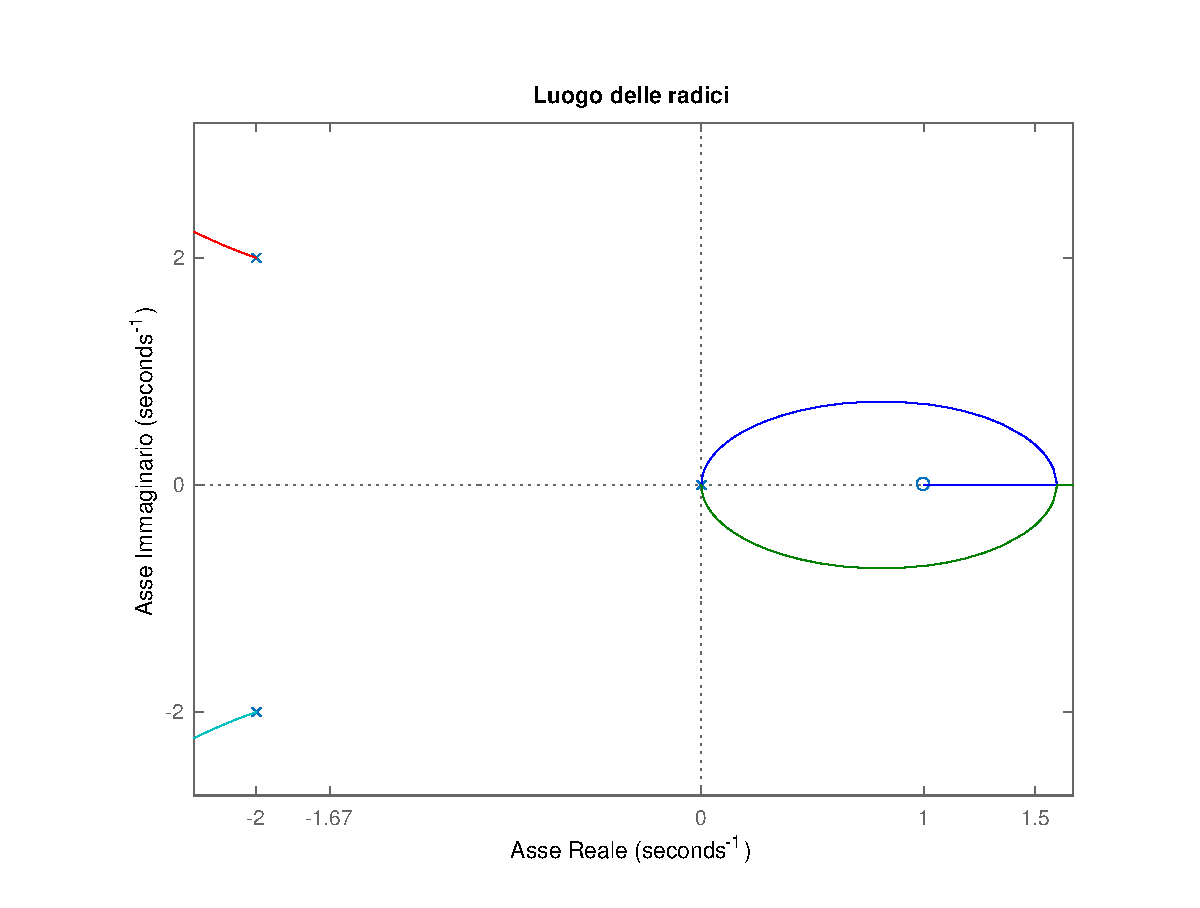
\includegraphics[scale=.5]{mod1/assets/rl_ex311n}
	\caption{per \(k<0\)}
\end{figure}

\begin{itemize}
	\item \emph{Asintoti}:
		\[
			\sigma_a = -\frac{5}{3} \qquad
			\theta_a = \frac{\Bigl(2\cdot\bigl[0,1,2\bigr]\Bigr)\pi}{3} = \Bigl[0,\frac{2}{3}\pi,\frac{4}{3}\pi\Bigr]
		\]
	\item \emph{Punti doppi}:
		\[
			k = -\frac{s^2\bigl((s+2)^2+4\bigr)}{s-1} \quad
			\text{per } s \in (-1,+\infty)
		\]
		\[\begin{array}{rr}
			\toprule
			s 	 & k 		\\
			\midrule
			1.3 	 & -83.88 	\\
			\bm{1.5} & \bm{-73.12} \\
			2 	 & -80 		\\
			\bottomrule
		\end{array}\]
		Per \(s=1.5\) si ha un punto doppio di \emph{confluenza}.
	\item \emph{Stabilità}: per \(k<0\) il sistema è \emph{instabile} con
		2 poli instabili.
\end{itemize}


\subsection{Esercizio}
Sia data la seguente funzione di trasferimento:
\[
	G(s) = \frac{s+4}{s(s^2+2s+2)}
\]
Determinare il luogo delle radici per \(k>0\).

\paragraph{Soluzione}

\begin{figure}[ht]
	\centering
	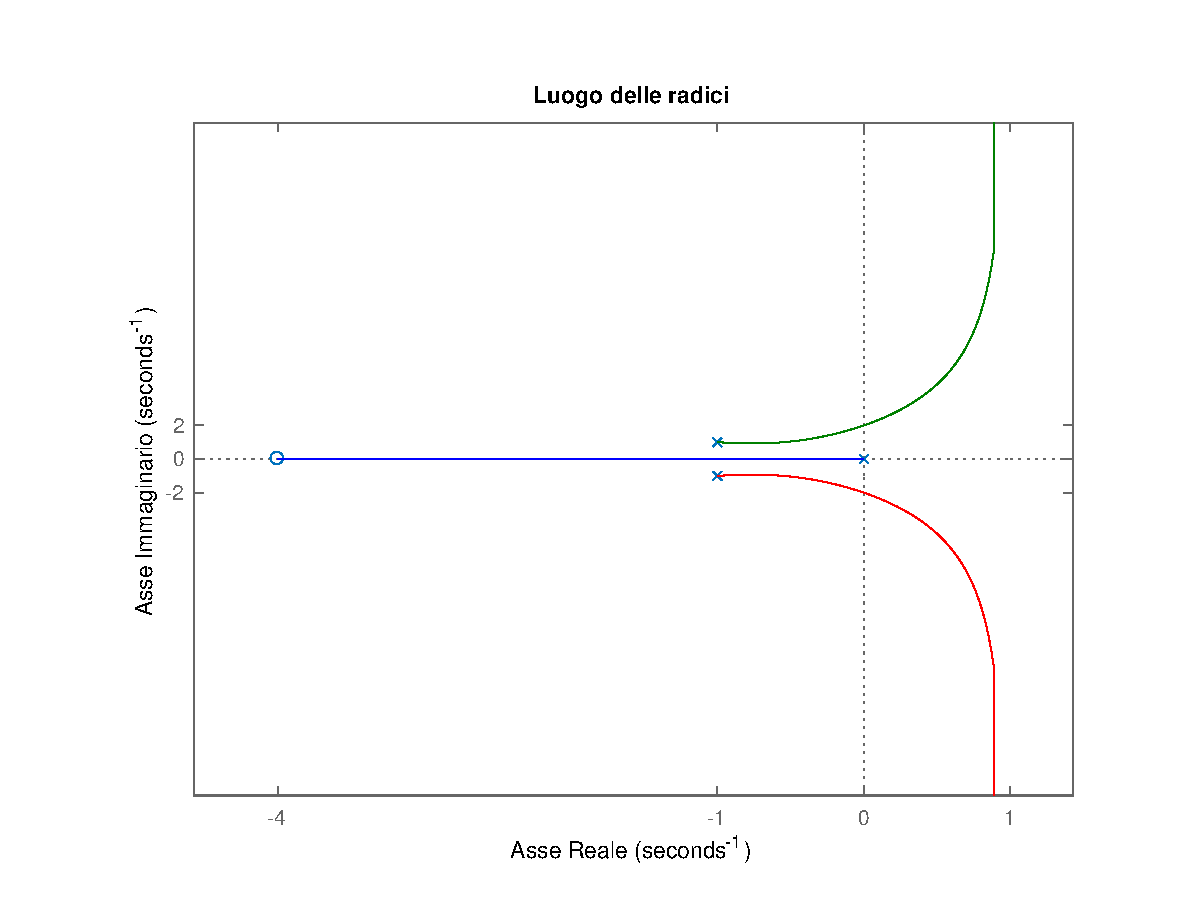
\includegraphics[scale=.6]{mod1/assets/rl_ex312}
\end{figure}

\begin{itemize}
	\item \emph{Punti di singolarità}:
		\begin{itemize}
			\item poli: \(\bigl\{-1\pm\jmath,0\bigr\}\)
			\item zeri: \(\bigl\{-4\bigr\}\)
		\end{itemize}
	\item \emph{Asintoti}:
		\[
			\sigma_a = \frac{-2\pm\jmath+4}{2} = 1 \qquad
			\theta_a = \frac{\Bigl(2\cdot\bigl[0,1\bigr]+1\Bigr)\pi}{2} = \Bigl[\frac{\pi}{2},\frac{3}{2}\pi\Bigr]
		\]
	\item \emph{Intersezioni con l'asse immaginario}:
		\[
			P(s) = s^3 + 2s^2 +(2+k)s +4k
		\]
		\[\begin{array}{r|rr}
			s^3 & 1 & 2+k 	   \\
			\bm{s^2} & 2 & 4k  \\
			s^1 & \bm{2-k} 	   \\
			s^0 & 4k
		\end{array}\]
		Per \(k=2\): \(2s^2+8=0 \rightarrow s=\pm\jmath2\)
	\item \emph{Angoli di partenza} per \(s=-1\pm\jmath\):
		\begin{align*}
			\varphi_- &= \pi +\angle(-1-\jmath+4) -\angle(-1-\jmath+1-\jmath) -\angle(-1-\jmath) = \\
				  &= \pi +\arctan{-\frac{1}{3}} +\frac{\pi}{2} -\arctan{1} +\pi = \\
				  &= 2\pi +\frac{\pi}{2} -0.322 -\frac{\pi}{4} = \SI{0.463}{\radian} \\
			\varphi_+ &= \pi +\angle(-1+\jmath+4) -\angle(-1+\jmath+1+\jmath) -\angle(-1+\jmath) = \\
				  &= \pi +\arctan{\frac{1}{3}} -\frac{\pi}{2} -\arctan{-1} -\pi = \\
				  &= -\frac{\pi}{2} +\frac{\pi}{4} +0.322 = \SI{-0.463}{\radian}
		\end{align*}
	\item \emph{Stabilità}:
		\[\begin{cases}
			k = 0\colon & \text{sistema \emph{semplicemente stabile}} \\
			0 < k < 2\colon & \text{sistema \emph{asintoticamente stabile}} \\
			k = 2\colon & \text{sistema \emph{semplicemente stabile}} \\
			k > 2\colon & \text{sistema \emph{instabile} con 2 poli instabili}
		\end{cases}\]
\end{itemize}

\subsection{Esercizio}
Sia data la seguente funzione di trasferimento:
\[
	G(s) = \frac{s-6}{s(s^2+4s+13)}
\]
Determinare il luogo delle radici per \(k>0\) e \(k<0\).

\paragraph{Soluzione per \(k>0\)}

\begin{figure}[ht]
	\centering
	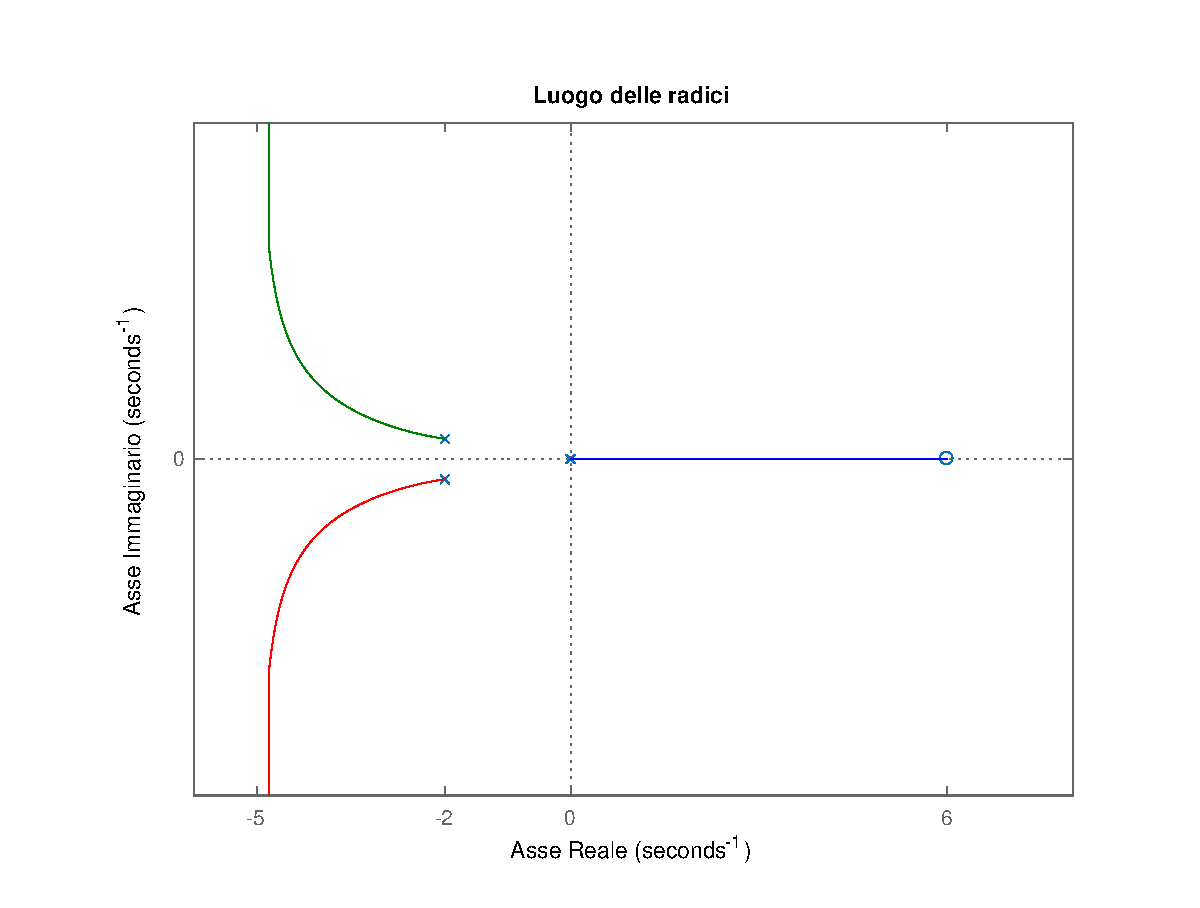
\includegraphics[scale=.5]{mod1/assets/rl_ex313}
	\caption{per \(k>0\)}
\end{figure}

\begin{itemize}
	\item \emph{Punti di singolarità}:
		\begin{itemize}
			\item poli: \(\bigl\{-2\pm\jmath3,0\bigr\}\)
			\item zeri: \(\bigl\{6\bigr\}\)
		\end{itemize}
	\item \emph{Asintoti}:
		\[
			\sigma_a = \frac{-4\pm\jmath3-6}{2} = -5 \qquad
			\theta_a = \frac{\Bigl(2\cdot\bigl[0,1\bigr]+1\Bigr)\pi}{2} = \Bigl[\frac{\pi}{2},\frac{3}{2}\pi\Bigr]
		\]
	\item \emph{Stabilità}:
		\[\begin{cases}
			k=0\colon & \text{sistema \emph{semplicemente stabile}} \\
			k>0\colon & \text{sistema \emph{instabile} con 1 polo instabile}
		\end{cases}\]
\end{itemize}

\paragraph{Soluzione per \(k<0\)}

\begin{figure}
	\centering
	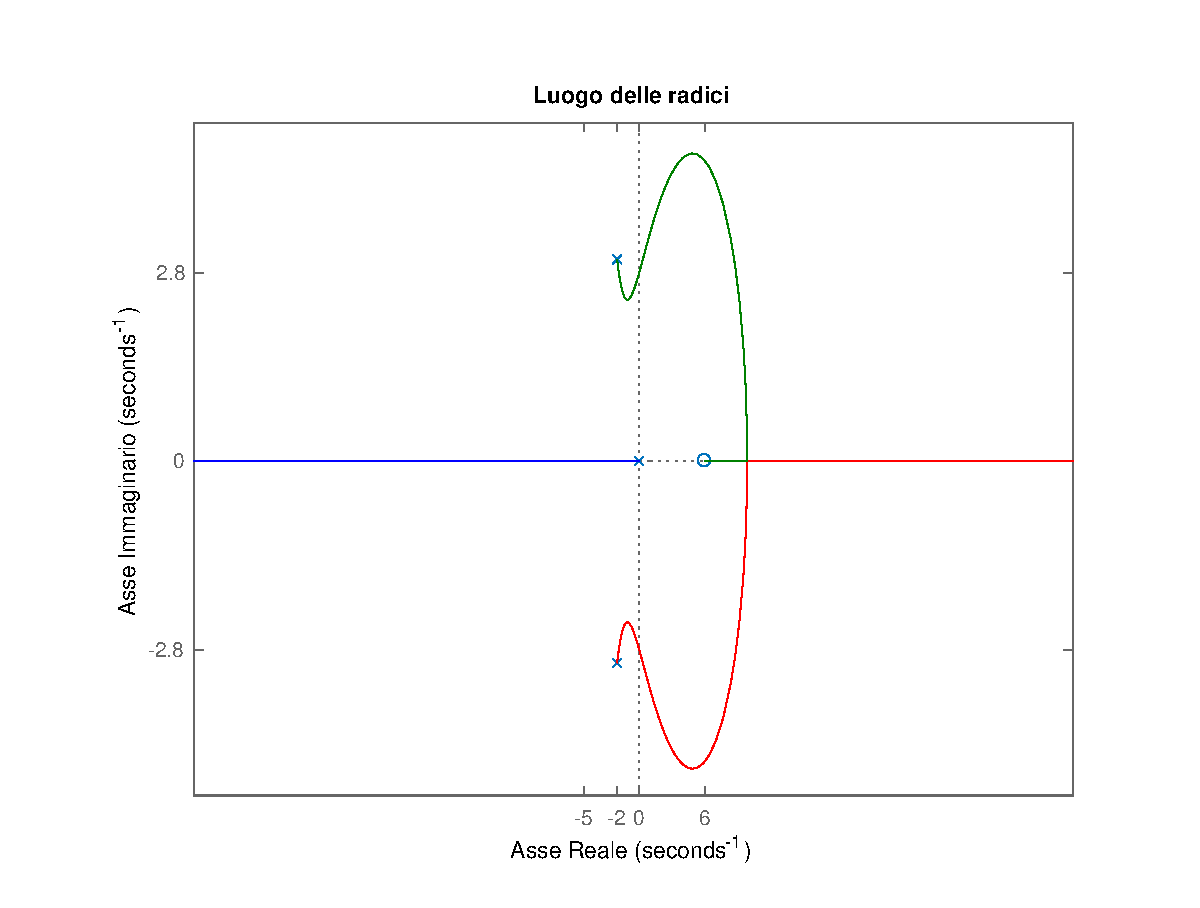
\includegraphics[scale=.5]{mod1/assets/rl_ex313n}
	\caption{per \(k<0\)}
\end{figure}

\begin{itemize}
	\item \emph{Asintoti}:
		\[
			\sigma_a = -5 \qquad
			\theta_a = \frac{2\cdot\bigl[0,1\bigr]\pi}{2} = \bigl[0,\pi\bigr]
		\]
	\item \emph{Punti doppi}:
		\[
			k = -\frac{s\bigl((s+2)^2+9\bigr)}{s-6} \quad
			\text{per } s \in (6,+\infty)
		\]
		\[\begin{array}{rr}
			\toprule
			     s &         k \\
			\midrule
			     8 &      -436 \\
			\bm{9} & \bm{-390} \\
			    10 &      -918 \\
			\bottomrule
		\end{array}\]
		Per \(s=9\) si ha un punto doppio di \emph{confluenza}.
	\item \emph{Angoli di partenza} per \(s=-2\pm\jmath3\):
		\begin{align*}
			\varphi_- &= \angle(-2-\jmath3-6) -\angle(-2-\jmath3+2-\jmath3) -\angle(-2-\jmath3) = \\
				  &= \arctan{\frac{3}{8}} -\pi +\frac{\pi}{2} -\arctan{\frac{3}{2}} +\pi = \\
				  &= \frac{\pi}{2} +0.359 -0.983 = \SI{0.946}{\radian} \\
			\varphi_+ &= \angle(-2+\jmath3-6) -\angle(-2+\jmath3+2-\jmath3) -\angle(-2+\jmath3) = \\
				  &= \arctan{-\frac{3}{8}} +\pi -\frac{\pi}{2} -\arctan{-\frac{3}{2}} -\pi = \\
				  &= -\frac{\pi}{2} -0.359 +0.983 = \SI{-0.946}{\radian}
		\end{align*}
	\item \emph{Intersezioni con l'asse immaginario}:
		\[
			P(s) = s^3 +4s^2 +(13+k)s -6k
		\]
		\[\begin{array}{r|rr}
			s^3 & 1 & 13+k \\
			s^2 & 4 & -6k  \\
			s^1 & 26+5k    \\
			s^0 & -6k
		\end{array}\]
		Per \(k = -\frac{26}{5}\) si ha \(4s^2+\frac{4\cdot39}{5}=0 \rightarrow s=\pm\jmath\sqrt{\frac{39}{5}}\).
	\item \emph{Stabilità}:
		\[\begin{cases}
			k < -\frac{26}{5}\colon & \text{sistema \emph{instabile} con 2 poli instabili} \\
			k = -\frac{26}{5}\colon & \text{sistema \emph{semplicemente stabile}} \\
			-\frac{26}{5} < k < 0\colon & \text{sistema \emph{asintoticamente stabile}}
		\end{cases}\]
\end{itemize}

\subsection{Esercizio}
Sia data la seguente funzione di trasferimento
\[
	G(s) = \frac{s-1}{(s+1)^4}
\]
Determinare il luogo delle radici per \(k>0\).

\paragraph{Soluzione}

\begin{figure}[ht]
	\centering
	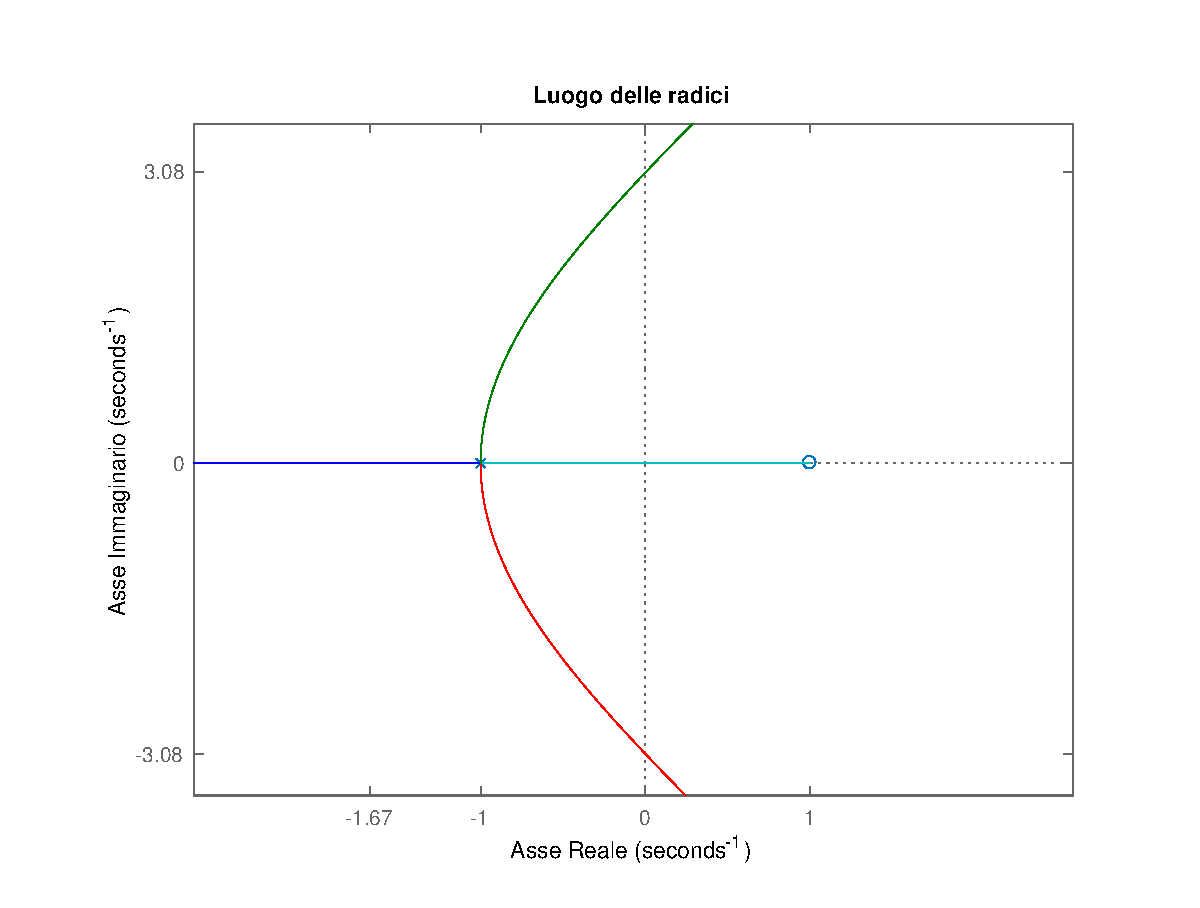
\includegraphics[scale=.6]{mod1/assets/rl_ex314}
\end{figure}

\begin{itemize}
	\item \emph{Punti di singolarità}:
		\begin{itemize}
			\item poli: \(\bigl\{-1\,[\times 4]\bigr\}\)
			\item zeri: \(\bigl\{1\bigr\}\)
		\end{itemize}
	\item \emph{Asintoti}:
		\[
			\sigma_a = \frac{4(-1)-1}{3} = -\frac{5}{3} \qquad
			\theta_a = \frac{\Bigl(2\cdot\bigl[0,1,2\bigr]+1\Bigr)\pi}{3} = \Bigl[\frac{\pi}{3},\pi,\frac{5}{3}\pi\Bigr]
		\]
	\item \emph{Intersezioni con l'asse immaginario}:
		\[
			P(s) = (s+1)^4 +ks -k = s^4+4s^3+6s^2+(4+k)s+1-k
		\]
		\[\begin{array}{r|rrr}
			s^4 & 1 & 6 & 1-k \\
			s^3 & 4 & 4+k \\
			\bm{s^2} & 20-k & 4-4k \\
			s^1 & \bm{-k^2+32k+64} \\
			s^0 & \bm{1-k}
		\end{array}\]
		Considerando
		\begin{align*}
			& k^2-32k-64=0 \\
			\rightarrow & k_1 = 16+8\sqrt{5} \\
			\rightarrow & (20-16-8\sqrt{5})s^2 +4-4(16+8\sqrt{5}) =0 \\
			\rightarrow & s=\pm\jmath\sqrt{\frac{15+8\sqrt{5}}{1-2\sqrt{5}}}
		\end{align*}
		Si nota inoltre che per \(k=1\) il sistema è \emph{semplicemente stabile}.
	\item \emph{Stabilità}:
		\[\begin{cases}
			0 \leq k < 1\colon & \text{sistema \emph{asintoticamente stabile}} \\
			k = 1\colon & \text{sistema \emph{semplicemente stabile}} \\
			1 < k \leq 16+8\sqrt{5}\colon & \text{sistema \emph{instabile} con 1 polo instabile} \\
			k > 16+8\sqrt{5}\colon & \text{sistema \emph{instabile} con 3 poli instabili}
		\end{cases}\]
\end{itemize}

\subsection{Esercizio}
Sia data la seguente funzione di trasferimento:
\[
	G(s) = \frac{s+z}{s+p}
\]
Determinare \(z,p\) tale che il sistema sia asintoticamente stabile.

\paragraph{Soluzione}
Il sistema per poter esistere deve esser tale che \(p\neq0\).
Per \(p<0\) si hanno poli instabili, per \(p>0\) invece poli stabili, ovvero con
\(\Re s<0\).
Se \(z<0\), il sistema diventerebbe instabile ad un certo valore \(k\).

Quindi il sistema è essere asintoticamente stabile quando
\[
	z,p > 0
\]

\subsection{Esercizio - Appello Gennaio 2017}
\begin{center}\begin{tikzpicture}[auto,node distance=2cm,>=latex']
	\node [input] (U) {};
	\node [sum,right of=U] (sum) {};
	\node [block,right of=sum,node distance=1.5cm] (GC) {\(G_C(s)\)};
	\node [block,right of=GC] (GP) {\(G_P(s)\)};
	\node [output,right of=GP] (Y) {};
	\draw [->] (U) -- node[pos=0] {\(U(s)\)} (sum);
	\draw [->] (sum) -- (GC);
	\draw [->] (GC) -- node[pos=0.5,name=sym] {} (GP);
	\draw [->] (GP) -- node[pos=0.5,name=retro] {\(Y(s)\)} (Y);
	\node [block,below of=sym,node distance=1.5cm] (H) {\(H(s)\)};
	\draw [->] (retro) |- (H);
	\draw [->] (H) -| node[pos=0.9] {\(-\)} (sum);
\end{tikzpicture}\end{center}

\subsubsection{
Siano \(\displaystyle G_P(s) = \frac{s+1}{s(s-5)(s+5)}\) e \(H(s) = 1\). \\
Supponendo \(G_C(s)=k\), si tracci e si orienti il luogo delle radici del sistema complessivo per \(k>0\) e \(k<0\), determinando i punti del luogo sull'asse reale, il centroide e gli asintoti, i punti doppi e i punti di incontro con l'asse immaginario con i corrispondenti valori di \(k\), ove presenti.
}

\paragraph{Soluzione per \(k>0\)}
\begin{itemize}
	\item Punti di singolarità: \begin{itemize}
		\item poli: \(\set{-5,0,5}\)
		\item zeri: \(\set{-1}\)
	\end{itemize}
	\item Mappa poli-zeri e luogo delle radici:
	\item Asintoti: \begin{itemize}
		\item \(\displaystyle \sigma_a = \frac{0+5-5+1}{2} = \frac{1}{2}\)
		\item \(\displaystyle \theta_a = \frac{\qty(2\qty[0,1]+1)\pi}{2} = \qty[\frac{\pi}{2},\frac{3}{2}\pi]\)
	\end{itemize}
	\item Punti doppi: ne prevedo uno in \(\qty(0,5)\). Uso la \emph{tabella di taratura}:
		\[\begin{array}{rr}
			\toprule
			s & k \\
			\midrule
			1.5 & 13.65 \\
			\bm{2} & \bm{14} \\
			2.5 & 13.39 \\
			\bottomrule
		\end{array}\]
		Quindi per \(s=2\) si ha un punto di \emph{emergenza}.
	\item Intersezioni con l'asse immaginario: per \(k=0\) si ha un polo nell'origine.
\end{itemize}

\paragraph{Soluzione per \(k<0\)}
\begin{itemize}
	\item Mappa poli-zeri e luogo delle radici:
	\item Intersezioni con l'asse immaginario: per \(k=0\) si ha un polo nell'origine.
\end{itemize}

\subsubsection{
Sempre nell'ipotesi \(G_C(s)=k\), si discuta la stabilità del sistema in anello chiuso al variare del parametro \(k>0\) e \(k<0\), specificando per quali valori è rispettivamente asintoticamente stabile, semplicemente stabile, o instabile (in caso di instabilità si precisi il numero di poli instabili).
}

\begin{itemize}
	\item Per \(k=0\) il sistema è \emph{instabile} con 1 polo a parte reale positiva e un polo nell'origine;
	\item per \(k>0\) il sistema è \emph{instabile} con 2 poli a parte reale positiva;
	\item per \(k<0\) il sistema è \emph{instabile} con 1 polo a parte reale positiva.
\end{itemize}

\subsubsection{Determinare il valore di \(k\) per cui esiste un polo in anello chiuso di valore \(s=-3\)}

\[k = -\frac{1}{G(-3)} = 24\]

\subsubsection{Per il valore di \(k\) determinato, individuare sul luogo la porzione dei rami in cui sono posizionati gli altri due poli.}

Dato che per \(s\approx2\), \(k\approx24\), gli altri due poli devono per forza trovarsi dopo il punto di emergenza, in direzione per gli asintoti.

\subsection{Esercizio - Appello Gennaio 2017}
\begin{center}\begin{tikzpicture}[auto,node distance=2cm,>=latex']
	\node [input] (U) {};
	\node [sum,right of=U] (sum) {};
	\node [block,right of=sum,node distance=1.5cm] (GC) {\(G_C(s)\)};
	\node [block,right of=GC] (GP) {\(G_P(s)\)};
	\node [output,right of=GP] (Y) {};
	\draw [->] (U) -- node[pos=0] {\(U(s)\)} (sum);
	\draw [->] (sum) -- (GC);
	\draw [->] (GC) -- node[pos=0.5,name=sym] {} (GP);
	\draw [->] (GP) -- node[pos=0.5,name=retro] {\(Y(s)\)} (Y);
	\node [block,below of=sym,node distance=1.5cm] (H) {\(H(s)\)};
	\draw [->] (retro) |- (H);
	\draw [->] (H) -| node[pos=0.9] {\(-\)} (sum);
\end{tikzpicture}\end{center}

\subsubsection{
Con riferimento alla figura, siano \(G_C(s)=k\), \(\displaystyle G_P(s)=\frac{s+3}{(s+1)^2(s+p)}\) e \(H(s)=s+2\) con \(k>0\) e \(p>0\). Si definisce l'errore come \(e(t)=u(t)-3y(t)\). \\
Dopo aver calcolato la funzione di trasferimento \(G_0(s)\) del sistema in anello chiuso, se ne verifichi la stabilità nelle ipotesi \(k>0\) e \(p>0\).
}

\begin{align*}
	G_0(s) &= \frac{G_C(s)G_P(s)}{1+G_C(s)G_P(s)H(s)} = \frac{\frac{k(s+3)}{(s+1)^2(s+p)}}{1+\frac{k(s+3)}{(s+1)^2(s+p)}(s+2)} = \\
	&= \frac{k(s+3)}{(s+1)^2(s+p)+k(s+3)(s+2)}
\end{align*}
Il sistema è \emph{asintoticamente stabile} per \(k>0\) e \(p>0\).

\subsubsection{Si determini la relazione che deve intercorrere tra i parametri \(p\) e \(k\) affinché si abbia un errore di posizione \(e_P=0.1\)}

\begin{align*}
G_{eq}(s) &= \frac{\gamma G(s)}{1+G(s)\qty(H(s)-\gamma)} = \frac{\frac{3k(s+3)}{(s+1)^2(s+p)}}{1+\frac{k(s+3)}{(s+1)^2(s+p)}(s+2-3)} = \\
&= \frac{3k(s+3)}{(s+1)^2(s+p)+k(s+3)(s-1)} = \frac{3k(s+3)}{(s^2+2s+1)(s+p)+ks^2+3ks-ks-3k} = \\
&= \frac{3k(s+3)}{s^3+2s^2+s+ps^2+2ps+p+ks^2+2ks-3k} = \\
&= \frac{2k(s+3)}{s^3+(2+p+k)s^2+(1+2p+2k)s+p-3k}
\end{align*}
Il sistema è di \emph{tipo 0}.
\[k_P = \lim_{s\to0} G_{eq}(s)=\frac{9k}{p-3k} \implies e_P=\frac{1}{1+k_P}=\frac{p-3k}{p+6k}=0.1=\frac{1}{10} \implies \bm{p=4k}\]
\chapter{Errori a regime}

\section{Esercizi svolti}
\begin{esercizio}
Siano dati
\[
	G(s) = \frac{2}{s^2+2} \qquad H(s) = s+2 \qquad e(t) = u(t) -3y(t)
\]
Si determinino \(e_p, e_v, e_a\).

\paragraph{Soluzione}
Si osserva che la retroazione \emph{non è unitaria}. Questo significa che si ha un errore \(\gamma\) ed è specificato tra i dati come il coefficente di \(y(t)\) in \(e(t)\) (altrimenti sarebbe stato \(\gamma = H(0)\)): quindi \(\gamma = 3\).
A questo punto è possibile ricavare \(G_{eq}(s)\) per poter poi procedere con gli errori:
\begin{align*}
	G_{eq}(s) &= \frac{\gamma G(s)}{1+G(s)\bigl(H(s)-\gamma\bigr)} =
			\frac{\frac{6}{s^2+2}}{1+\frac{2}{s^2+2}\bigl(s+2-3\bigr)} =
			\frac{\frac{6}{s^2+2}}{\frac{2^2+2+2s-2}{s^2+2}} =
		  	\frac{6}{s(s+2)}
\end{align*}
e si osserva che il sistema è \emph{di tipo 1} perché ha un polo nell'origine.
Posso procedere con gli errori di posizione, velocità e accelerazione:
\begin{align*}
	k_p &= \lim_{s\to0} G_{eq}(s) = \lim_{s\to0} \frac{6}{s(s+2)} = +\infty \implies e_p = \frac{1}{k_p} = 0 \\
	e_v &= \lim_{s\to0} \frac{1}{s G_{eq}(s)} = \lim_{s\to0} \frac{s(s+2)}{6s} = \frac{1}{3} \\
	e_a &= \lim_{s\to0} \frac{s^2 G_{eq}(s)} = \lim_{s\to0} \frac{s(s+2)}{6s^2} = +\infty
\end{align*}
\[\implies \begin{cases}
	e_p = 0 \\
	e_v = \frac{1}{3} \\
	e_a = +\infty
\end{cases}\]
\end{esercizio}

\begin{esercizio}
Siano dati
\[
	G_c(s) = k \qquad G_p(s) = \frac{1}{s(s+4)} \qquad H(s) = 1
\]
Si determini quando il sistema è \emph{asintoticamente stabile}, il valore di \(k\) tale che \(e_v = 0.1\) e \(e_p\), \(e_a\).

\paragraph{Soluzione}
Per la stabilità ricorro a \(G_0(s)\):
\begin{align*}
	G_0(s) &= \frac{G(s)}{1+G(s)H(s)} \quad \text{con } G(s) = G_c(s)G_p(s) \\
	\implies G_0(s) &= \frac{\frac{k}{s(s+4)}}{1+\frac{k}{s(s+4)}} =
		\frac{\frac{k}{s(s+4)}}{\frac{s(s+4)+k}{s(s+4)}} =
		\frac{k}{s^2+4s+k}
\end{align*}
Noto che per \(k>0\) i coefficienti sono tutti positivi, quindi per il \emph{Lemma di Routh} il sistema è asintoticamente stabile per \(k>0\).

Dato che il sistema è a retroazione unitaria:
\begin{align*}
	G_{eq}(s) &= G(s) = \frac{k}{s(s+4)} \longrightarrow \text{sistema di \emph{tipo 1}} \\
	&\implies \begin{cases}
		e_p = 0 \\
		e_v = \frac{4}{k} = 0.1 \implies k=40 \\
		e_a = +\infty
	\end{cases}
\end{align*}
\end{esercizio}

\begin{esercizio}
Siano dati
\[
	G_c(s) = k \qquad G_p(s) = \frac{s+3}{(s+1)^2(s+p)} \qquad
	H(s) = s+2 \qquad e(t) = u(t) -3y(t)
\]

\paragraph{Verifica la stabilità del sistema.}
\[
	G_0(s) = \frac{G(s)}{1+G(s)H(s)} =
		\frac{\frac{k(s+3)}{(s+1)^2(s+p)}}{1+\frac{k(s+3)}{(s+1)^2(s+p)}(s+2)} =
		\frac{k(s+3)}{(s+1)^2(s+p)+k(s+3)(s+2)}
\]
Per il \emph{Lemma di Routh} il sistema è asintoticamente stabile per \(k>0,\,p>0\).

\paragraph{Stabilire la relazione tra \(p\) e \(k\) tale che \(e_p = 0.1\).}
\begin{align*}
	G_{eq}(s) &= \frac{\gamma G(s)}{1+G(s) \bigl(H(s) - \gamma\bigr)} \quad
			\text{con } \gamma = 3 \\
	G_{eq}(s) &= \frac{\frac{3k(s+3)}{(s+1)^3(s+p)}}{1+\frac{k(s+3)}{(s+1)^3(s+p)}(s+2-3)} = \\
		  &= \frac{3k(s+3)}{(s+1)^3(s+p)+k(s+3)(s-1)} \;
			\longrightarrow \text{sistema di \emph{tipo 0}} \\
	k_p &= \lim_{s\to0} G_{eq}(s) = \frac{9k}{p-3k} \\
	\implies e_p &= \frac{1}{1+k_p} = \frac{1}{1+\frac{9k}{p-3k}} = \frac{p-3k}{p-3k+9k} = \frac{p-3k}{p+6k} = \frac{1}{10} \\
	\implies p &= 4k
\end{align*}

\paragraph{Verificare se esiste una relazione tra \(p\) e \(k\) tale che \(e_v\) ed \(e_a\) siano finiti.}
\[
	G_{eq}(s) = \frac{3k(s+3)}{(s+1)^3(s+p)+k(s+3)(s-1)} = \frac{3k(s+3)}{s^3 +(p+2+k)s^2 +(1+2p+2k)s +p-3k}
\]
Per far sì che \(e_v\) sia finito, il sistema deve essere di tipo 1, quindi \(p-3k=0 \rightarrow p = 3k\). Per far sì che \(e_p\) sia finito, il sistema deve essere di tipo 2, quindi \(1+2p+2k=0\). Ponendo a sistema le equazioni:
\[\begin{cases}
	p = -\frac{3}{8} \\
	k = -\frac{1}{8}
\end{cases}\]
\(p<0\), \(k<0\), quindi la relazione non è valida.
\end{esercizio}

\begin{esercizio}
Siano dati
\[
	G_c(s) = 1 \qquad G_p(s) = \frac{10}{s(s+10)} \qquad
	H(s) = h > 0 \qquad e(t) = u(t) -hy(t)
\]
\paragraph{Determinare \(h\) tale che \(e_v\leq0.2\).}
Si nota che la retroazione è \emph{parametrica}, quindi si deve porre \(G_{eq}(s)=hG(s)\).
\begin{align*}
	G_{eq}(s) &= hG(s) = \frac{10h}{s(s+10)} \longrightarrow \text{sistema di \emph{tipo 1}} \\
	e_v &= \lim_{s\to0} \frac{1}{1+sG_{eq}(s)} =
		\lim_{s\to0} \frac{1}{1+s\frac{10h}{s(s+10)}} = \\
	    &= \lim_{s\to0} \frac{s+10}{s+10+10h} =
	    	\frac{1}{h} \leq \frac{1}{5}
	    	\rightarrow h \geq 5
\end{align*}

\paragraph{Con \(h=5\) stabilire il valore a regime, il valore massimo di sovraelongazione e il tempo di picco.}
.
\end{esercizio}


% TODO: Prima parte - prima dell'esonero di aprile
\chapter{Sintesi o progettazione del regolatore}
\end{document}
